\documentclass[12pt,preprint]{aastex}
\usepackage{url}
\usepackage{natbib}
\usepackage{graphicx}
\usepackage{subfig}
\usepackage{appendix}
\usepackage{gensymb}
\usepackage{amsmath}
%\usepackage{algorithmic}
\usepackage{algpseudocode}

%\usepackage{fixltx2e}



%%%%%%%%%%%%%%%%%%%%%%%%%%%%%%%%%%%%%%%%%%%%%%%%%%%%
%%% author-defined commands
\newcommand\x         {\hbox{$\times$}}
\def\mic              {\hbox{$\mu{\rm m}$}}
\def\about            {\hbox{$\sim$}}
\def\Mo               {\hbox{$M_{\odot}$}}
\def\Lo               {\hbox{$L_{\odot}$}}

%\captionsetup[figure]{labelformat=simple}
%%%%%%%%%%%%%%%%%%%%%%%%%%%%%%%%%%%%%%%%%%%%%%%%%%%%

% Abstract




\begin{document}

\title{Moving Object Pipeline System Design}

\author{Jonathan Myers, Lynne Jones, Tim Axelrod}

\begin{abstract}

The Moving Object Pipeline System (MOPS) has two responsibilities
within LSST Data Management.  First, it is responsible for generating
and managing the \textbf{Moving Object} data products.  The Moving
Objects are identified solar system objects with associated Keplerian
orbits, errors, and detected sources associated with those solar
system objects.  The second responsibility of the MOPS is to predict
future locations of moving objects in incoming images so that their
sources may be associated with known objects; this will reduce the
number of transient detections and prevent Alert Generation on
detections of known Solar System objects.  

\end{abstract}

\tableofcontents
\listoffigures

\section{System Design and Responsibilities}

The Moving Object Pipeline System has two main responsibilities: the
generation and maintenance of the Moving Object database, and the
prediction of known object locations which are sent to the Association
Pipeline to prevent unneccessary alerts.  The MOPS has been broken
into two components, colloquially known as ``DayMOPS'' and ``NightMOPS.''
 

\begin{figure}[!ht]
\centering
  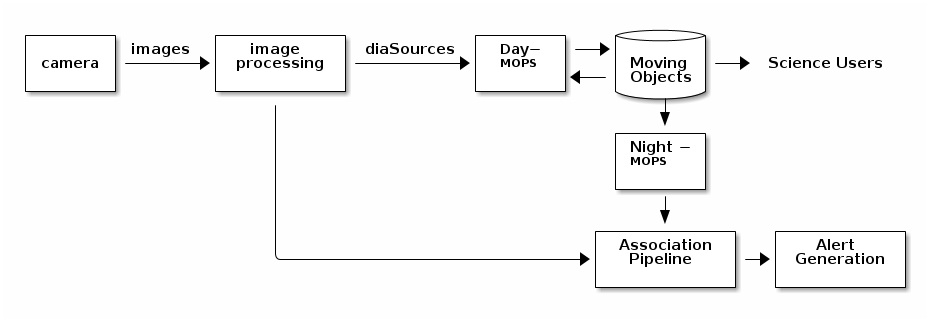
\includegraphics[width=13cm]{illustrations/mopsWithinLsst.png}
\caption{ Data flow from the camera through DayMOPS to the Science
  Users and Alert Generation.  DayMOPS will build and maintain the
  Moving Objects table, NightMOPS will use the Moving Objects table to
  communicate with the Assocation Pipeline.  }
\label{mopsWithinLsst}
\end{figure}


``DayMOPS,'' so called because it processes data acquired from the
previous night in a large batch operation, is responsible for
discovering new Moving Objects in newly-acquired data, searching old
data for detections of new objects, and updating the Moving Objects
table to reflect newly-acquired data. It is also responsible for
periodically cleaning and refining the contents of the Moving Objects
table.  ``NightMOPS'' is responsible for projecting the locations of known
Moving Objects in upcoming images as they are announced during
night-time operations.  

The relationship between DayMOPS, NightMOPS and the neighboring
components of the LSST Data Management system is illustrated in
figure \ref{mopsWithinLsst}.

\subsection{DayMOPS: Discovering and Managing Moving Objects}

% Illustration of DayMOPS

% sky-plane vs. orbit-space illustration

The DayMOPS is responsible for discovering moving objects in source
catalogs.  The task of discovering and tracking asteroids has been
performed by humans since hundreds of years ago, but automated systems
for asteroid discovery and tracking remain relatively uncommon.  Other
surveys have often mixed human and computerized approaches -
\textbf{can we get some more history here?}.


The design of the LSST DayMOPS is based on the PanSTARRS Moving Object
Pipeline System \citep{psMOPSDesign}.  The approach used here is to
first find sets of detections with sky-plane paths consistent with
asteroid behaviour; these sets of detections and their fitted paths
are called \textbf{tracks}.  A set of algorithms for the discovery of
sky-plane tracks in dense data are presented in
\citet{Kubica:2005:MTA:1081870.1081889}; these algorithms are the
basis of the linking methods for the current LSST DayMOPS.


%% TBD: it would be really nice to have some illustrations here
%% showing detections of an object, and possibly tracklets and tracks
%% as well

The tracking methods used are based on a tiered approach; first two or
more detections from a single night are linked into
\textbf{tracklets}, which represent a hypothetical object and a linear
approximation of its sky-plane motion.  These tracklets are later
joined into larger tracks. Because of the increasing complexity of
sky-plane motion over time, we are generally interested in tracks
which span no more than 15-30 days of observation time.

The PanSTARRS MOPS uses a fairly loose and generous approximation of
asteroid motion.  This allows for many mislinkages or \textbf{false
  tracks}, combining detections which are not attributable to the same
source, but virtually all objects for which a true (correctly-linked)
track could be generated will get some correct track.  With LSST's
expected density of detections, we found that this glut of false
tracks was generally too painful.  As a result, our methods diverge
from those of PanSTARRS as we introduce some more strict filters on
tracks, reducing the number of mislinkages at the expense of
potentially missing some true tracks.  The algorithms, their
implementations, the additional filters, and their behaviors are
presented thoroughly in Chapter \ref{linking}.

Once tracks are discovered, they are sent to the Orbit Determination
phase. The Orbit Determination phase takes these sets of sky-plane
detections and attempts to find a Keplerian orbit which could generate
the detections.  This orbit is further refined, and error bounds are
established, using differential correction.  Orbit Determination will
reject many tracks as false, but should successfully find precise
orbits for virtually all correctly linked tracks.  Several methods for
performing this task are known, and several have open-source implementations
available to LSST \citep{Milani04orbitdetermination},
\citep{Milani2006}, \citep{OpenOrb2009}, \citep{granvik_thesis}.  The
orbits discovered by Orbit Determination, and the detections present
in the track associated with each orbit, are used to generate new
Moving Objects.

\begin{figure}[h]
\begin{center}
  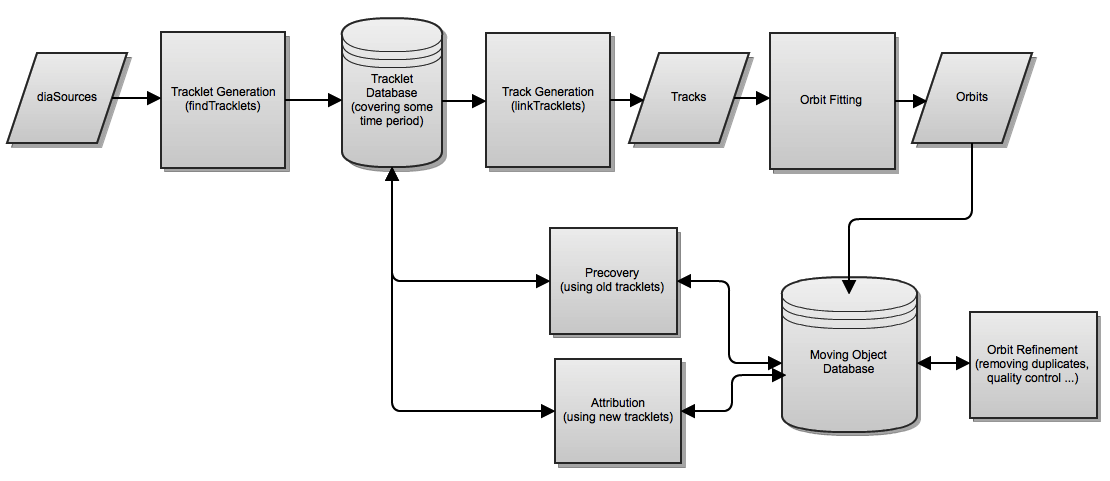
\includegraphics[width=11cm]{illustrations/mopsDiagram.png}
\end{center}
\caption{ Data flows into the DayMOPS pipeline and results in
  modifications of the Moving Objects table in a variety of ways,
  including attribution to known objects, a multi-stage pipeline for
  the discovery of new objects, and periodic refinements of the Moving
  Object table, such as possible merges of redundant objects or
  removal of false orbits. }
\label{mopsDiagram}
\end{figure}



The DayMOPS is expected to perform several additional tasks to manage
and improve the Moving Objects table over time.  Attribution is the
process of identifying known objects in incoming data and adding those
detections to the correct Moving Object, in a process called
Attribution. Similarly, Precovery is the recovery of known,
unattributed detections associated with a newly-discovered Moving
Object.  Another refinement is the merging of potentially redundant
Moving Objects.  The complete set of DayMOPS tasks and their data
flows are illustrated in figure \ref{mopsDiagram}.






%% nabbed from http://tex.stackexchange.com/questions/19982/how-do-i-add-parfor-in-algorithmic-environment
% declaration of the new block
\algblock{ParFor}{EndParFor}
% customising the new block
\algnewcommand\algorithmicparfor{\textbf{parfor}}
\algnewcommand\algorithmicpardo{\textbf{do}}
\algnewcommand\algorithmicendparfor{\textbf{end\ parfor}}
\algrenewtext{ParFor}[1]{\algorithmicparfor\ #1\ \algorithmicpardo}
\algrenewtext{EndParFor}{\algorithmicendparfor}


\section{The Linking Stages of DayMOPS}
\label{linking}

Sufficiently bright moving objects which are observed by the LSST
telescope will generate diaSource detections, stored in the LSST
diaSource detection catalog.  The LSST diaSource detection catalog
will also hold detections from a variety of non-moving object sources,
including transient phenomena and artifacts of image processing.  One
of the major responsibilities of dayMOPS is to link these diaSources
into tracklets and tracks, as described earlier (see
Section~\ref{daymopsOverview}). 


\subsection{Linear and Quadratic and more: Models of Motion}

\begin{figure}[ht]
  \centering
    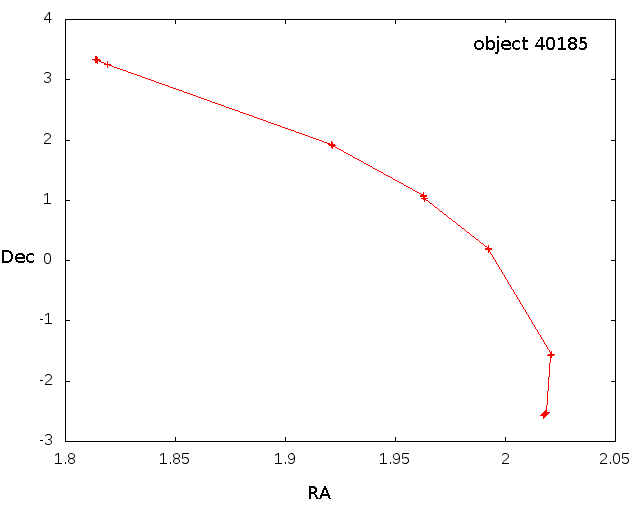
\includegraphics[width=10cm]{illustrations/4.png}
    \caption[Object motion across the sky.]{A plot of simulated observations of object 40185 on the
      sky.  Though the observations span only one week, a pronounced
      quadratic path is visible.  Note that the object is observed two
      or more times on each night.}
\label{objectMotion}
\end{figure}


In order to discover and identify new objects, astronomers have
traditionally used sky-plane approximations to predict and model the
behavior of solar system objects for which a true orbit is not yet
known.  As a general rule of thumb, objects are said to move linearly
(with a more or less fixed velocity) in RA and Dec over the course of
a single night and quadratically (having velocity and some
acceleration) in RA and Dec over the course of a month.  These are, of
course, approximations, and linear and quadratic fits will inevitably
contain some error.  An example of one object with a clear quadratic
path over seven days is show in Figure~\ref{objectMotion}.

In general, these approximations become closer to the actual sky-plane
motion of the object as objects are observed at larger distances from
the Earth or at solar elongations closer to opposition. It's worth
noting however, that for faster moving objects such as NEOs or objects
observed further from opposition, these approximations start to break
down; for example, NEOs do show acceleration over the course of a
night (although generally not significant acceleration over 90
minutes) and any moving object near turn-around (where its motion
appears to reverse direction on the sky) will provide a poor fit to
quadratic motion over a month.

These basic approximations are our starting point and are used to determine
which detections could plausibly be linked. For tracklets, this is
simple; diaSources which can be linked with linear motion become
tracklets. For tracks, however, first we determine which diaSources
could potentially be joined into tracks (using the velocity
information from the tracklets along the way) using quadratic motion,
but then this track undergoes some further scrutiny before being
marked as `valid'. 

When we are determining the validity of tracks, by looking at
residuals between the observed positions and the quadratic
approximation of motion (and rejecting detections or whole tracks
which do not have low enough residuals), we have found that allowing
for residuals high enough to account for errors due to the quadratic
approximation itself permits too many mislinkages. The discovery rate of
false tracks is hundreds of times the rate of discovering true tracks;
we become swamped with false detections. 

To avoid this, when determining the validity of a track, we now
require stricter tests.  The primary goal here is to reduce the
residuals to allow for tighter filtering of the potential tracks. The
first step is to attempt to add a topocentric correction to the
detections; during the night, as the Earth rotates, objects which are
close to Earth will have some additional `wiggle' in their motion due
to the change in observer's location.  A topocentric correction factor is
determined for each tracklet before building the kd-trees; when the potential
tracks are evaluated, we now fit for a topocentric correction to the observed 
positions -- the topocentric correction is the range (1/distance) times this topocentric 
correction factor. This additional parameter is fit using only the RA values,
as the effect in Declination is small. We also permit the use of a higher 
order polynomial to fit the detections, if it is supported by the track;
{\it i.e.} if the fit residuals are lower than all of the errors between the
predicted positions and the measured positions, the order
of the fit is too high. After the fit for the track is
created (always separately fit in RA/Dec), then a
chi-squared probability is computed for the track. We reject tracks
with chi-squared values larger than a predetermined cutoff; this
cutoff is determined experimentally to optimize the true / false track
ratio. 

Note that tracklets and tracks represent hypothetical linkages, many
of which may be incorrect.  The linking algorithms are greedy, and
intended to permit finding as many moving objects as possible. Thus, a
single detection may exist in several tracklets and/or several tracks
and a given tracklet may be found in multiple tracks, shown in
Figure~\ref{objectLinking}.  However, once a diaSource is linked into
an actual Orbit, it will not be joined into any further tracklets or
tracks or other moving objects. 


\begin{figure}[ht]
  \centering
    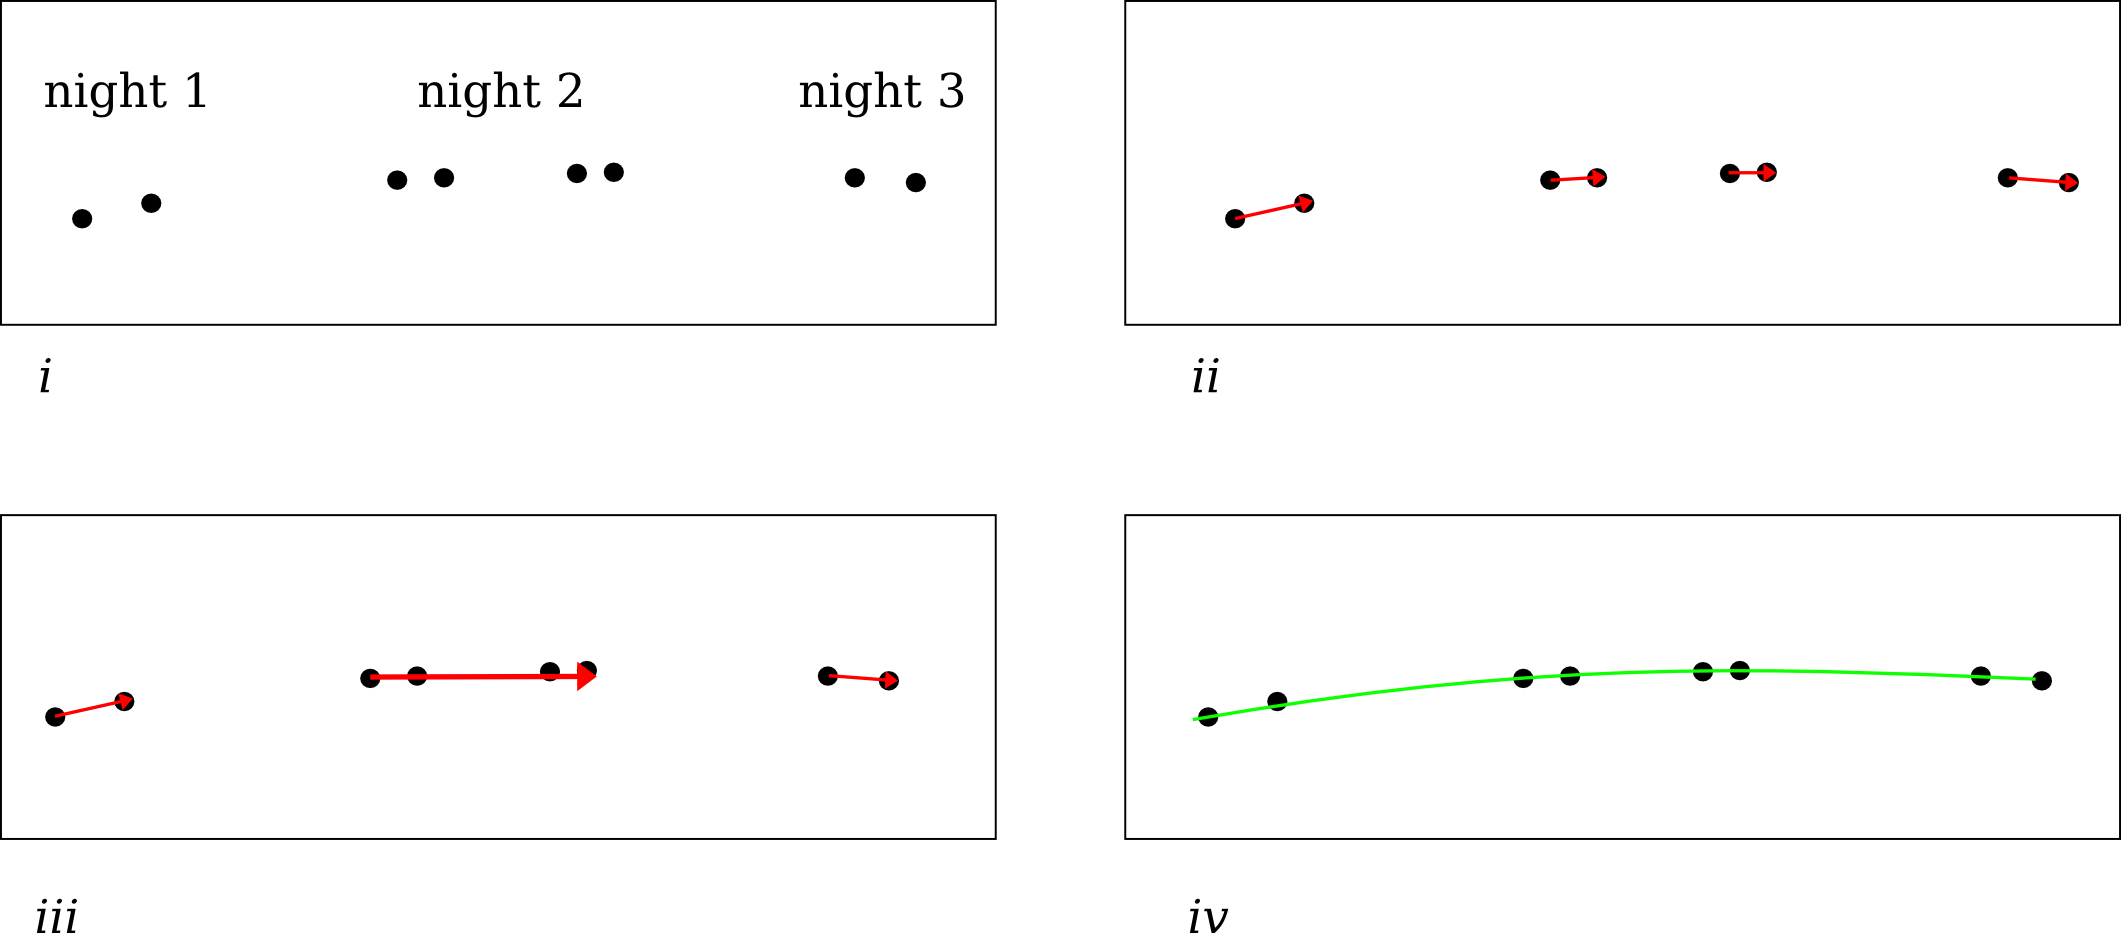
\includegraphics[width=16cm]{illustrations/oneObjectMops.png}
    \caption[Example dayMOPS linkages.]{An illustration of how DayMOPS linkage might be applied
      to a single object.  In $i$, the object is observed on three
      nights; on the first and last night, it gets two detections per
      night, but on the second night it gets four.  In $ii$, initial
      tracklets are generated; time separation of visits on the second
      night is such that we get two tracklets.  In $iii$, we merge the
      tracklets from the second night so there are only three
      tracklets.  In $iv$, we attempt inter-nightly linking and
      generate a single track.}
\label{objectLinking}
\end{figure}

%%%%%%%%%%%%%%%%%%%%%%%%
%%% findTracklets
%%%%%%%%%%%%%%%%%%%%%%%%%


\subsection{Building Tracklets : findTracklets}

\textbf{Tracklets} are linkages between DiaSource detections occuring
within the same night. By creating tracklets, DayMOPS can find
sky-plane position and velocity estimates for sets of detections which
may belong to the same solar system objects.  The use of tracklets
also simplifies the downstream work of track generation, which
attempts to find sets of detections with a good
position/velocity/acceleration fit on the sky-plane; since tracklets
have known position and velocity, the track generation phase needs
only to find those tracklets compatible within some acceleration
factor.

Correctly-linked tracklets from a given object are needed to generate
a good track for that object and eventually discover its orbit.
However, if these useful tracklets are too deeply buried among very
large numbers of other tracklets, then the job of tracklet linking
will become extremely slow and expensive.  Generally, these other,
unwanted tracklets are false tracklets (mislinkages between detections
not attributable to the same object), though in special conditions
large numbers of correctly-linked but redundant tracklets can cause
pain as well (this will discussed in \ref{collapseTracklets}).

In order to ensure that tracklet-generating images are acquired, it is
necessary to ensure that fields of the sky are visited two or more
times within an accepted time period each night. To constrain the
number of tracklets, we impose a maximum apparent velocity on the
tracklets, and also require that sky fields be revisited within a
fairly short time period ($\leq 90$ minutes is the current rule).
Raising the maximum velocity threshold enables one to find
faster-moving objects, and raising the maximum allowed revisit time
also enables one to generate tracklets in more fields of the sky;
however, increasing either of these thresholds also increases the
search space and can significantly increase the number of mislinked
tracklets, greatly increasing the cost downstream.

The process of initial tracklet creation is accomplished by the
findTracklets software.  Later refinement of tracklets is accomplished
by collapseTracklets and additional filters, primarily purifyTracklets. 

\subsubsection{Algorithm} 

The findTracklets software is responsible for finding pairs of
detections which occur within a fixed time threshold, and have
apparent velocity below a given threshold.  For a given detection and
a set of image times, one can calculate the maximum distance an object
could have travelled at each time using the velocity limit.  To find
detections with which the query detection could be linked, one can
imagine searching a circular region in the later images based on this
distance.

\begin{figure}[ht]
  \centering
    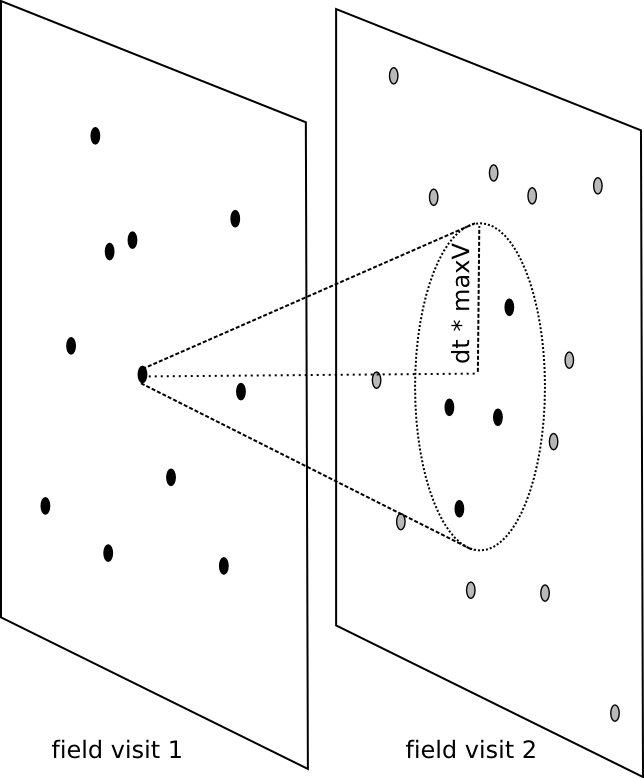
\includegraphics[width=6cm]{illustrations/findTracklets-onequery.png}
    \caption[An example of findTracklets endpoints.]{An example of searching for compatible second endpoints
      for a given detection.  The first detection and each of the
      second endpoints will be used to create a new tracklet.}
\label{findTrackletsIllustrated}
\end{figure}


This can be accomplished in a fairly straightforward way through the use of
KD-Trees.  KD-Trees are hierarchical data structures which allow for quickly and
efficiently performing range searches on points in space
\citep{bentley_kdtrees}.  We use KD-Trees for many different purposes
in MOPS, but what these uses have in common is exploiting the
hierarchical nature of the trees; using the fact that by checking the
boundaries at a high-level on a branch we may rule out having to
compare any of the data stored at lower levels on that
branch. 

A KD-Tree-based method for building
tracklets was first contributed by Jeremy Kubica for his PhD thesis
\citep{kubica_thesis}.  For findTracklets, 2-Dimensional KD-Trees are
used, covering the space of (RA, Dec).  Given a detection and trees
containing detections from later images, we can use range searches to
quickly find nearby detections in those later images and use them for
the creation of tracklets.


\begin{figure}[ht]
\hrulefill
\begin{algorithmic}[5]
\Require $I$ is a set of images, each of which has an associated exposure time and contains a set of detections
\State \Comment{Create a 2D KD-Tree for each image, holding detections from that image.}
\State $T \gets \emptyset$
\For {$i \in I$}
  \State $t \gets$ Make2DTree$(i.detections)$
  \State $t.time \gets i.time$
  \State $T \gets T \cup \{t\}$
\EndFor
\State \Comment{Use these trees to discover the actual tracklets.}
\State $tracklets \gets \emptyset$
\For {$t_1 \in T$}
  \State $later \gets \{t_i \in T : 0 < t_i.time - t_1.time < maxDt\}$
  \For{$d \in t_1.detections$}
     \For{$t_q \in later$}
 
       \State \Comment{Use time between images and max velocity to
         calculate the max travel distance}

        \State $dt \gets t_q.time - t_1.time$
        \State $dd \gets dt * maxV$
        \State \Comment{Use KD-Tree range search to find detections within max travel distance}
        \State $tracklets \gets tracklets \cup t_q.$rangeSearch($d.ra, d.dec, dd$)
     \EndFor
   \EndFor
\EndFor
\Return{$tracklets$}
\end{algorithmic}
\hrulefill
\caption[findTracklets psuedocode.]{Pseudo-code for the findTracklets algorithm.  2D (RA, Dec)
  trees are created for each image; for each detection, later trees
  are searched for nearby detections. }
 \label{findTrackletsAlgorithm}
\end{figure}


Because the sky is a sphere, notions of `distance' and `velocity' must
be handled carefully, especially near the poles.  Both the KD-Tree
library used and the findTracklets software use actual great-circle
distance and velocity for their queries, avoiding problems near the
poles.  The software should also be impervious to wrap-around errors -
objects which move between, say, $359.9 \degree$ in RA and $.01
\degree$ in RA will be detected.  The Appendix \ref{kdTreeLib}
explains the KD-Tree library used in greater detail.

The findTracklets software itself only finds pairs of diaSources which
could potentially be moving objects; if particular solar system object
was observed four times in one night, it could potentially generate
six separate tracklets, depending on the time of the observations and
the time limits imposed by findTracklets. 

%%%%%%%%%%%%%%%%%%%%%%%%%%%%%%%%%%%%%%%%%%%%%%%%%%%%%%%%%%%%%%%%%%5
%% COLLAPSE TRACKLETS & purify tracklets
%%%%%%%%%%%%%%%%%%%%%%%%%%%%%%%%%%%%%%%%%%%%%%%%%%%%%%%%%%%%%%%%%%5


\subsection{Merging Tracklets} \label{collapseTracklets}

Finding multiple tracklets for a single object makes later stages of
linking inefficient; if every object was observed four times per
night, the number of tracklets could be increased by a factor of six -
at both the start and endpoints of the tracks - resulting in a 36 times
increase in the number of output tracks. Observing fields of the sky
(and thus, generating multiple tracklets) more than twice in a night
is common with our current OpSim runs, and is actually desireable for
several purposes. In addition, the `Deep Drilling' fields observe fields many
more than twice per night. In fields observed $n$ times per night, the
number of tracklets can grow like $O(n^2)$, potentially generating
huge numbers of tracklets. Merging tracklets these tracklet pairs, as
appropriate, removes the inefficiencies for later stages of linking,
thus there are some post-findTracklets merging and filtering stages to
address this issue. 

The `collapseTracklets' software 
attempts to join colinear 2-detection tracklets into longer (3
detections or more) tracklets, while the `purifyTracklets' software
attempts to avoid the risk of merging mislinked with true tracklets.

In addition, it is sometimes possible that a tracklet may link
together a set of detections already present in another higher
cardinality (longer) tracklet; the `removeSubsets' software finds and
removes these shorter subsets. The subset removal algorithm can be
used for tracks as well as tracklets, and so is presented in
section~\ref{subsetRemoval} after the description of linkTracklets.


\subsubsection{CollapseTracklets} 

In collapseTracklets, a method similar to the Hough transform is used
to identify roughly colinear tracks and merge them. 
An intermediate time, $t_c$ is selected (we use the average time of
the first and last detections) and use the apparent linear motion of
the tracklets to project their location at $t_c$.  We then store these
projected (RA,Dec) locations and the angle/velocity of each tracklet.
At this point, colinear tracklets should have similar positions and
motion vectors, making them easy to find.  This is accomplished with a
series of range searches, which of course can be implemented with 4-D
(RA, Dec, angle, velocity) KD-Trees.  The full pseudo-code is
presented in Figure \ref{collapseTrackletsAlgorithm}.

More information on collapseTracklets is available in Jon Myer's
Master's thesis, titled `Methods for Solar System Object Searching in
Deep Stacks', submitted 2008 to the Dept of Computer Science at U of
Arizona. A PDF of this document is available in the LSST git
repository of dayMOPS/docs. 

Code and usage:  The collapseTracklets algorithm is implemented in {\tt
  collapseTracklets.h} and {\tt collapseTracklets.cc}.  A command-line
interface is implemented in {\tt collapseTrackletsMain.cc}.  Run {\tt
  collapseTracklets -h} for usage hints.

\begin{figure}[ht]
\hrulefill
\begin{algorithmic}[5]
  \Require $T$ is a set of intra-nightly tracklets, $D$ is the set of nightly detections from which $T$ was created, $range$ is a 4-tuple of tolerances for RA, Dec, angle and velocity.
  \State $t_c \gets midpoint(\{ d_{time} : d \in D \})$
  \For {$t \in T$}
    \State Calculate $t$'s predicted location at time $t_c$, its motion angle and velocity
  \EndFor
  \State \Comment{Create a 4D KD-Tree of the tracklets on their projected RA, Dec position and motion angle/velocity.}
  \State $tree \gets$ Make4DTree$(T)$
  \State $outTracklets = \emptyset$
  \For {$t \in T,\ t$ has not already merged with another tracklet}
    \State \Comment{Find tracklets with projected location, motion similar to that of $t$}
    \State $candidates \gets tree.$rangeSearch$(t_{projected\ position}, t_{angle}, t_{velocity}, range)$
    \For {$c \in candidates$} 
      \If{$c$ and $t$ do not contain different detections from the same image}
        \State $t.detections \gets t.detections \cup c.detections$
        \State mark $c$ as already merged
      \EndIf
    \EndFor
    \State mark $t$ as already merged
    \State $outTracklets \gets outTracklets \cup t$
  \EndFor
  \Return{$outTracklets$}
\end{algorithmic}
\hrulefill
\caption[collapseTracklets psuedocode.]{Pseudo-code for the collapseTracklets algorithm. A 4-D KD-Tree over RA, Dec, angle, velocity is constructed using the projected locations and motion of the tracklets.  Tracklets which are similar in this 4-D space are roughly colinear, so they are merged and written to output.}
\label{collapseTrackletsAlgorithm} 
\end{figure}

Issue: Currently, collapseTracklets handles wrap-around, but otherwise treats
the sky as a flat (RA, Dec) plane when calculating the projected
positions of tracklets.  This is acceptable for tracklets close to the
ecliptic, but not sufficient closer to the poles.  This should be
fixed when possible.

Issue: Choosing an appropriate set of thresholds for collapseTracklets may be
difficult; with variable time between images, the amount of error on
velocity may differ from tracklet to tracklet.  Other factors come
into play as well; higher thresholds will lead to more correct
linkages as well as more incorrect linkages - which, as described in
the following section, can be ``undone'' later by purifyTracklets.  We
arrived at our current thresholds through simple trial and
error. These threshholds will have to be evaluated for use with real
data with real astrometric errors and time variability. 

\subsubsection{PurifyTracklets}
PurifyTracklets examines the merged tracklets and removes detections
if they are sufficiently far from the best-fit line. The algorithm is
presented in Figure~\ref{purifyTrackletsAlgorithm}. 

\begin{figure}[ht]
\hrulefill
\begin{algorithmic}[5]
  \Require $T$ is a set of tracklets, $rmsMax$ is a maximum root-mean
  squared residual on the tracklet's best-fit function to its
  detections

  \For {$t \in T$}
    \State $rms = RMS(t)$
    \While {$rms > maxRms, |t| > 2$} 
      \State remove the worst-fitting detection from $t$
      \State $rms = RMS(t)$
    \EndWhile
  \EndFor
  \Return{$outTracklets$}
\end{algorithmic}
\hrulefill
\caption[purifyTracklets pseudocode.]{In purifyTracklets, poorly-fitted detections are ``pruned''
  from tracklets. In certain degenerate cases, we may prune tracklets
  down to only two detections, in which case the two-detection
  tracklet is kept.}
\label{purifyTrackletsAlgorithm}
\end{figure}





%%%%%%%%%%%%%%%%%%%%%%%%%%%%%%%%%%%%%%%%%%%%%%%%%%%%%%%%%%%%%%%%%%%%%
%%          LINKTRACKLETS
%%%%%%%%%%%%%%%%%%%%%%%%%%%%%%%%%%%%%%%%%%%%%%%%%%%%%%%%%%%%%%%%%%%%%


\subsection{Building Tracks: linkTracklets}

With tracklets already assembled, we should have many linkages
representing the position, location, and velocity of the various
objects observed, as well as ``false'' mislinked tracklets.  While
tracklets have only linear motion, tracks have more complex paths; in the
track building phase, this is always calculated as a pair of quadratic
functions in RA and Dec, rather than a single motion vector.  By
making use of this quadratic approximation of motion, valid for
approximately one month, we can move a sliding window of up to 30 days
over the data, looking for tracklets which could be linked by some
quadratic acceleration factor.  As we find these linkages, depending
on the individual detections themselves, we will also calculate a topocentric correction to the
detections and a higher-order fit in order to apply a stronger
requirement on the residuals to the fit when outputting tracks. 

Generally, the track generation phase is the most computationally
resource intensive task in DayMOPS processing. Unlike other stages,
which consider only a night's-worth of data at a time, it must
consider tracklets from many nights and find linkages between them. In
order to build a useful track, suitable for orbit fitting, we need to
link tracklets from three separate nights, within our sliding window
of time (generally we use 15 days for this time window, to make the
computations manageable). 
In general, this task scales exponentially with the number of
tracklets, the time between observations, and the velocity limits for the
tracklets. Thus it can quickly become overwhelming with dense source
data, high velocity and acceleration limits, poor merging of
tracklets, and long time windows.  

To tackle this problem, we use an algorithm for performing this track
discovery presented by Kubica et al. (\citet{kubica_thesis},
\citet{Kubica:2005:MTA:1081870.1081889}).  In essence, the idea behind
the algorithm is to build per-image 4D-Trees of (RA position, Dec
position, RA velocity, Dec velocity), and use these to hold the
tracklets, indexed by position/velocity.  We then imagine the KD-Trees
as hierarchical bounding boxes, and consider pairs of bounding boxes
from different nights, calculating whether they could be linked by
some acceleration factor less than our maximum acceleration threshold.
If the boxes could be linked, then a track may exist within their
contents and we continue searching bounding boxes lower in the tree
hierarchy; if not, we know that no track of interest to us could pass
through the boxes and we can abandon searching immediately.  By using
the hierarchical structure of the KD-Trees, we can avoid searching in
large areas of tracklet-space where no track could ever exist, greatly
reducing our workload. While these are similar to the KD-trees used in
findTracklets, they are more complex because of the higher
dimensionality (4D instead of 2D) and there are many more trees
involved (each individual image is
represented by a tree instead of one tree for an entire night's data,
as in findTracklets). 

\subsubsection{Recursive Tree-walk Using Pruning}
\label{searchPruning}

In the linkTracklets algorithm, all tracklets starting in a given
image are placed in a single 4D-Tree containing bounding boxes in (RA
position, Dec position, RA velocity, Dec velocity)-space.  One tree is
created for each of the images. It is then possible to calculate the
acceleration needed for an object in one bounding box in one tree to
reach ({\it i.e.} be compatible with) the second bounding box in a
later tree.  Because we are generally interested in tracks which have
acceleration within a fixed range (e.g. between $>.02 deg/day^2$ and
$<-.02 deg/day^2$), we can abandon searching at a given pair of
bounding boxes if the necessary acceleration is outside our range of
interest.

The minimum and maximum acceleration connecting two bounding boxes is
currently calculated as follows:

\begin{equation}
maxAcc = \min  \left(\begin{array}{ccc} & \displaystyle \frac{Node2.maxV - Node1.minV}{dt} \\
& \displaystyle \frac{2}{dt^2} \bigg(Node2.maxP_0 - Node1.minP_0 - Node1.minV \times dt \bigg) \\
& \displaystyle \frac{2}{dt^2} \bigg(Node1.maxP_0 - Node2.minP_0 + Node2.maxV \times dt \bigg) \end{array}\right)
% & \displaystyle parentMaxAcc, \\ jeremy says this shouldn't happen, even though it's in the code
\label{maxAcc}
\end{equation}

\begin{equation}
minAcc  = \max  \left(\begin{array}{ccc} & \displaystyle \frac{Node2.minV - Node1.maxV}{dt},\\
& \displaystyle \frac{2}{dt^2} \bigg( Node2.minP_0 - Node1.maxP_0 - \displaystyle Node1.maxV \times dt\bigg), \\
& \displaystyle \frac{2}{dt^2} \bigg(Node1.minP_0 - Node2.maxP_0 + Node2.minV \times dt\bigg) \end{array} \right)
%   & parentMinAcc, jeremy says this shouldn't happen, even though its in the code.
\label{minAcc}
\end{equation}


Issue: Note that this approach simplifies the problem by treating the sky as
a flat plane, which will be problematic near the poles.  However, the
above calculation appears to be the ``hot spot'' of the linkTracklets
algorithm and accounts for most of the computation time, and so
simplifying to reduce floating point costs greatly improves
performance.

In the code, this calculation is performed by the function 
{\tt updateAccBoundsReturnValidity} in {\tt linkTracklets.cc}.

Pruning allows the rapid avoidance of searching in areas where no track
can exist. As a simplified introduction to the
full algorithm, see Figure~\ref{simplifiedLinkTracklets} for a
two-tracklet-linking, ``endpoint-only'' version of the algorithm which
finds pairs of compatible tracklets on different nights.

\begin{figure}[ht!]
\hrulefill
\begin{algorithmic}[5]
  \Require{$nodeA$ and $nodeB$ are KD-Tree nodes which hold tracklets
    from two different images on different nights, $minAcc$ and $maxAcc$
    specify the limits of accelerations which the user finds
    interesting.}
  
  \State $accRange = $ min/max acceleration to move from $nodeA$ to $nodeB$
  \If{$accRange$ does not overlap $(minAcc, maxAcc)$}
  \Return $\emptyset$
  \Else
  \If{$nodeA$ and $nodeB$ are leaf nodes}
  
  \State \Comment{When we hit a pair of terminal nodes, and their
    acceleration bounds are interesting, then we have found a set
      of tracklets which may be sufficient to create a track.}
    
    \Return $\{$tryToBuildATrack($nodeA$.tracklet, $nodeB$.tracklet)$\}$
    \Else
    
    \State \Comment{In order to ensure that this function sees
      nodes which are roughly the same size, we choose the larger
      node and ``split'' that one, recursing on its children.}


    \State $largerNode, smallerNode \gets orderBySize(nodeA, nodeB)$
    \State $leftRes \gets recurse(largerNode.\text{leftChild}, smallerNode, S)$
    \State $rightRes \gets recurse(largerNode.\text{rightChild}, smallerNode, S)$
    \Return $ leftRes \cup rightRes $
    \EndIf
    \EndIf    
  \end{algorithmic}
\hrulefill
  \caption[Simplified linkTracklets pseudocode.]{An endpoint-matching, two-tracklet version of the
    linkTracklets algorithm.  Note that if two nodes have no chance at
    holding a compatible tracklet (first ``if'' check) then their
    children are never searched; only if they may hold an interesting
    track are the children searched.  In this way, the algorithm
    avoids even examining a great number of KD-Tree node pairs and
    thus the pairs tracklets contained therein.}
  \label{simplifiedLinkTracklets}
\end{figure}

\paragraph{Support Tracklets, Support Nodes, and the Full LinkTracklets Algorithm}

For orbit determination, we require detections on at least three separate
nights.  The endpoint-only algorithm in \ref{simplifiedLinkTracklets}
will only attempt to find pairs of tracklets, giving tracks with only
two nights of observational data.  In practice, we seek to find tracks
with tracklets from three unique nights.  This could be accomplished
using various extensions to the endpoint-only algorithm, but it is
argued in \citet{kubica_thesis} and
\citet{Kubica:2005:MTA:1081870.1081889} that by far the most efficient
of these variants is called the algorithm called the {\bf vtrees} (for
``variable trees'') algorithm.

In the vtrees algorithm, we search for tracks with one or more
intermediate ``support'' tracklets in between the ``endpoint'' or
``model'' tracklets (the first and last tracklet).  To accomplish
this, the vtrees algorithm searches for compatible endpoint nodes as
in Figure~\ref{simplifiedLinkTracklets} but, as search progresses, maintains
a list of compatible ``support'' nodes - nodes which could hold useful
intermediate tracklets between the tracklets in the endpoint nodes.
These are filtered at each step, again using the equations
\ref{maxAcc} and \ref{minAcc}.  As the search descends through the
possible valid combinations of endpoint nodes, the support list is
filtered and refined.  When search terminates at a pair of leaf nodes,
the support nodes are used to find possible support tracklets.  If the
support list ever becomes empty, we can prune the searching at this
point, since we know no useful track (no track with at least three
nights of data) could exist between the endpoint
nodes.

The full vtrees algorithm is presented in
Figure~\ref{linkTrackletsAlgorithm}.  This is the actual algorithm
implemented by the function {\tt doLinkingRecurse} from {\tt linkTracklets.cc}


\begin{figure}[ht!]
\hrulefill
\begin{algorithmic}[5]
\Require{$nodeA$ and $nodeB$ are KD-Tree nodes which hold tracklets
  from two different images on different nights, $S$ holds a series of
  nodes from images take on nights in between $nodeA.time$ and
  $nodeB.time$, $minAcc$ and $maxAcc$ specify the limits of
  accelerations which the user finds interesting.}

\State $accRange = $ min/max acceleration to move from $nodeA$ to $nodeB$
\If{$accRange$ does not overlap $(minAcc, maxAcc)$}
    \Return $\emptyset$
  \Else
  
  \For{$supportNode \in S$}
  \If{$supportNode$ represents an awkwardly large portion of tracklet-space relative to $nodeA$ and $nodeB$}
    \State replace $supportNode$ with $supportNode.rightChild$ and $supportNode.leftChild$, coming back to them later
    \Else
    \If{no track with acceleration within $accRange$ could pass from $nodeA$ through $supportNode$ and into $nodeB$}
      \State remove $supportNode$ from $S$
    \EndIf
  \EndIf

  \If{$S$ is empty}
    \Return $\emptyset$ \Comment{There is no way to build a three-tracklet track using the contents of these nodes, so abandon searching.}
  \EndIf

  \EndFor
    \If{$nodeA$ and $nodeB$ are leaf nodes}

    \State \Comment{Again, try to build a track, this time using $S$ for intermediate tracklets}

       \Return $\{$tryToBuildATrack($nodeA$.tracklet, $nodeB$.tracklet, $S$)$\}$
    \Else

       \State $largerNode, smallerNode \gets orderBySize(nodeA, nodeB)$
       \State $leftRes \gets recurse(largerNode.\text{leftChild}, smallerNode, S)$
       \State $rightRes \gets recurse(largerNode.\text{rightChild}, smallerNode, S)$
       \Return $ leftRes \cup rightRes $
  \EndIf
\EndIf

\end{algorithmic}
\hrulefill
\caption[linkTracklets pseudocode.]{The full vtrees algorithm, the actual algorithm implemented
  in linkTracklets.  At each recursion, $S$, the set of support nodes,
  is split based on the position, velocity, and acceleration range
  implied by the $nodeA$ and $nodeB$, the two endpoint nodes.  Note
  that if support nodes are periodically ``split'' and replaced with
  their chidlren if they too large relative to $nodeA$ and $nodeB$.}
 \label{linkTrackletsAlgorithm}
\end{figure}

In the algorithm, support nodes are filtered and possibly split (and
their children filtered) at each recursive step.  Choosing when to
split the support nodes is an important performance question.  If we
split too aggressively, then we will add more items to $S$ and be
required to filter a larger number of nodes at each recursion, which
will increase cost at each step.  If we split support nodes too
rarely, then the support nodes may become very large relative to the
endpoint nodes and we will often find that we have some compatible
support node, and thus continue searching - even in cases where, had
we split the support nodes, we would have seen that none of the leaf
nodes held by the larger box were consistent with our
position/velocity/acceleration range.  This leads to needless
searching when we should have simply terminated.

Currently, the cutoff for splitting is based on the spatial size of
the support node relative to that of the two endpoint nodes.  First
a weighting factor, $\alpha$, is calculated:

\begin{equation}
\alpha = \frac{supportNode.time - nodeA.time}{supportNode.time - nodeB.time}
\end{equation}

We then split the node if, for \textit{any} of the spatial axes (RA position, Dec position, RA velocity, or Dec velocity):

\begin{equation}
\bigg(\frac{width(nodeA.axis)}{\alpha} + \alpha \x width(nodeB.axis)\bigg) < 4 \x width(supportNode.axis)
\end{equation}

Where $width$ is the spatial extent of the node.  This approach was
developed by Jeremy Kubica through empirical testing, and may or may
not be optimal for our data; however, in our experience, it seems to
be effective.

The splitting and filtering of the support trees is implemented by
{\tt splitSupportRecursively} in {\tt linkTracklets.cc}.  This
function uses several helper functions, including the same {\tt
  updateAccBoundsReturnValidity} function used to check the
compatibility of endpoint nodes.


\subsubsection{Track Validation}

Once a pair of endpoint tracklets and one or more support tracklets
have been found via the vtrees algorithm, we may attempt to finally
build a track from them.  This is relatively straightforward; three or
more tracklets with compatible acceleration, from three or more
nights, have already been found.  However, this acceleration factor is
rather approximate, as it is based on the position and velocity
estimate of the tracklets, not the best-fit to the detections held in
the tracklet.  Thus, at this point we actually start examining the
detections themselves.

The track fitting is conducted in the method {\tt
  calculateBestFitQuadratic} in {\tt Track.cc}. First the Dec values
of the observations are fit to either a quadratic or higher order
(despite the name of the method) function, using the residuals of the
fit compared to the differences between predicted and actual positions to
control the order of the fit. Then the RA values of the observations
are fit, with the added complication of including a topocentric
correction (essentially fitting for the range of the object). 
The order of the function in Dec and RA do not have to be the same.  

In the event there are multiple possible support detections at one of
these image times, the best-fitting detection is chosen. 

After the fit is determined, the chi-squared probability of the RA and
Dec fits is calculated for the `chi-squared probability filter'.  If
an insufficient number of valid detections are found or the
chi-squared probability of the RA or Dec fits is higher than the
predetermined cutoff, the potential track is rejected.  If it is
validated, then it is passed to the set of output tracks.

\subsubsection{Issues and Quirks}
\label{someLinkingIssues}

\paragraph{Topocentric Correction}
We can generate more precise fits and do more aggressive filtering if we fit for a
topocentric correction to the detections, basically converting from topocentric
coordinates to geocentric coordinates. For this reason, before the positions/velocities of the
tracklets are calculated, the trees are built or the linking algorithm
is run, a topocentric correction factor is calculated for each
tracklet - this is the topocentric correction for an object at 1 AU observed at the times 
of the detections in the tracklet. When the RA values of the potential track are fit, the appropriate 
topocentric correction (which is the topocentric correction factor multiplied by the range, or 1/distance)
is fit for at the same time as a higher order polynomial. The order of this polynomial is variable,
depending on what the track will support, in terms of predicted positions vs. observed measurements and their 
expected astrometric error. 

Issue: This topocentric correction fit should be verified over the entire sky, as it was developed for
use near the equator/ecliptic. 

Note: if it holds up, this could be a useful tool for orbit fitting as well. 


\paragraph{Spherical Geometry Issues}
Currently, the tracklet tree constructor in {\tt TrackletTree.cc} will
alter RA (and if needed, Dec) values so that all RA (and possibly Dec)
values are stored on a contiguous 180-degree region.  This simplifies
the critical ``hot-spot'' calculations in {\tt
  updateAccBoundsReturnValidity}, since we do not need to check for
values which cross over the 0/360 line in RA.  However, this means
that if the input data covers too large an area of the sky then the
acceleration range calculation will likely fail, and thus the whole
algorithm will misbehave.

Further, as mentioned in section \ref{searchPruning}, we simplify the
math throughout track generation by treating the sky as a flat plane,
which will lead to significant distortion near the poles.  This
problem is often addressed by rotating the data in question so that it
is centered on the RA, Dec origin (0,0), where polar distortions are
minimal.  This could be done for the entire input set of detections,
but if the detections cover a sufficiently large area of the sky then
we will not significantly reduce the problem.  Temporarily
re-centering the relevant points at each call to {\tt
  updateAccBoundsReturnValidity} would likely work, but would probably
be quite expensive.  This is a problem which needs to be addressed
eventually, perhaps by changing the equations used in
\ref{searchPruning}, or per by rotating the bounding boxes per-query,
so that the endpoint images will always be roughly centered over the
origin.

Issue: Due to manpower constraints, we have not been able to test how big a problem this is, if
the acceleration calculations are failing, and to what degree assuming
the sky is `flat' is distorting acceleration and compatibility
calculations.  It might be interesting to look at placing these trees
into a x/y/z/vx/vy/vz sphere instead of the current RA/Dec/vRA/vDec
coordinates. It is worth remembering that most of our tests have been
using 15 day windows, so over most of the sky we will not have
detections that cover much more than 180 degrees in RA except
potentially near the poles. 


\paragraph{Special Considerations of KD-Tree Construction for linkTracklets} 

Astrometric error on detections will affect both the position and
velocities of true tracklets.  As a result, bounding boxes must be
extended to encompass not just the tracklets which they hold, but the
surrounding error bars.  Each tracklet will have a unique error bar on
its velocity, as tracklets will span different distances in RA and Dec
($dp$) and may also span different numbers of images and thus have
different $dt$:

\begin{eqnarray}
minV = (dp - 2\times astrom\_err)/dt  \\
maxV = (dp + 2\times astrom\_err /dt
\end{eqnarray}

Thus, each node in the tracklet KD-Tree will have its position range extended by:

\begin{eqnarray}
minP_0 = P_0 - astrom\_err \\
maxP_0 = P_0 + astrom\_err  
\end{eqnarray}
\\ and its velocity range will be extended to encompass the $minV$ and
$maxV$ of all its child tracklets.  These rules apply to leaf nodes as
well as non-leaf nodes, which must have bounds at least as great as
their child nodes.  Note that as a result of expanding the boxes
around tracklets, KD-Tree nodes may actually overlap.

Note that for linkTracklets, a leaf node's bounds should only extend
as far as the error bars around their tracklets, and the non-leaf
nodes should encompass only the area around their children's bounds.
One of our early implementations did not follow this rule, and instead
partitioned the space in a ``top-down'' fashion as in the left side of
Figure~\ref{trackletTree}, and it then handled the issue of error bars
in the acceleration calculation function.  This was technically
correct, but lead to horrific performance - 1,000 or 10,000 times
slower than the current version, illustrated on the right side of
Figure~\ref{trackletTree}.  This is because the earlier version had
nodes which encompassed larger areas of tracklet-space and thus sets
of nodes were more likely to appear compatible, which results in less
search pruning.

\begin{figure}[ht!]
\centering
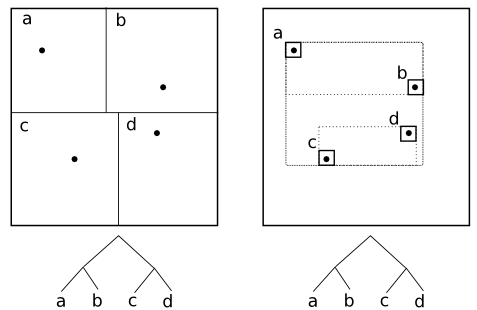
\includegraphics[width=10cm]{illustrations/kdTree_trackletTree.png}
\caption[KD-tree construction example.]{Two possible ways of
  constructing a KD-Tree over four points. The left shows a top-down
  tree; the right shows a tree constructed from the bottom up and with
non-leaf branches extending only as far as their children's bounds. }
\label{trackletTree}
\end{figure}

The former type of tree is simpler to construct (and perhaps easier to
visualize when debugging).  This is the type of tree used in most the
other algorithms, which perform range searches and thus can extend
handle their error bars per-query by extending their ranges as needed.
However, the latter type of tree is the one needed for linkTracklets,
and is implemented by the KD-Tree subclass {\tt TrackletTree} in {\tt
  TrackletTree.cc}.


\paragraph{Performance Enhancements for Acceleration Range Calculation}
As noted earlier, the function {\tt updateAccBoundsReturnValidity},
which implements the equations \ref{maxAcc} and \ref{minAcc},
accounts for most of the CPU time spent in linkTracklets.  Thus,
optimizing performance in this section of code is critical.

Rather than evaluate all arguments to $\min$ and $\max$ functions at
the outset, the code attempts to evaluate each possible argument. If
it becomes clear at any point that $minAcc > maxAcc$, then
we know that the search can be pruned and the function returns
immediately.

As an additional optimization, we start with $minAcc$ and $maxAcc$ set
to the values used by our caller in the recursive searching. We know
that the caller was examining two endpoint nodes which were either
equal to or a parent of our current nodes, and thus our parents
$(minAcc, maxAcc)$ range will be greater than the one we
calculate. (For the initial start of the recursion, we use the
user-specified min/max acceleration thresholds, because we do not care
about any values outside this range anyway.)  By doing this, we
actually have a $maxAcc$ value available as soon as we calculate our
first possible $minAcc$ value and vice-versa; this allows the earliest
possible termination.  However, it does make the code somewhat more
confusing to read.

This confusion is somewhat amplified by the fact that this same {\tt
  updateAccBoundsReturnValidity} function is used for filtering
support nodes.  In this case, the initial $minAcc$ and $maxAcc$ values
are taken from the acceleration range calculated when examining the
endpoint nodes $nodeA$ and $nodeB$, since we are not interested in
finding acceleration values which connect $nodeA$ and a support node
unless they also connect the support node to $nodeB$.

This is not an issue, just an explanation of the reasoning for
including $minAcc$ and $maxAcc$ values from the parent and endpoint
nodes. 





%%%%%%%%%%%%%%%%%%%%%%%%%%%%%%%%%%%%%%%%%%%%%%%%%%%%%%%%%%%%%%%%%%%%%%%%
%%      TRACK FILTERING
%%%%%%%%%%%%%%%%%%%%%%%%%%%%%%%%%%%%%%%%%%%%%%%%%%%%%%%%%%%%%%%%%%%%%%%%
\subsection{Subset Removal}
\label{subsetRemoval}

Some tracks are {\bf subset tracks} of other tracks; that is,
occasionally detections linked by one track found by linkTracklets
will be a subset of those linked by another track in the same output
set.  This can arise for a variety of reasons, but occurs most
commonly when a real object generates tracklets on four or more nights
within a linking period. We generally expect that these subset tracks
are unhelpful, and because they increase the size of the set of tracks
sent to orbit determination, they are possibly costly.

Finding and removing subset tracks could be accomplished with a very
naive double-for loop over the set of tracks, but of course this does
not scale to larger data sets ($O(n^2)$ for $n$ tracks).  A more
efficient algorithm uses a detection-to-track ``reverse-map'' $R$,
which maps from each detection to the set of tracks holding that
detection.  This is easy to construct for a set of tracks $T$:

\hrulefill
\begin{algorithmic}[5]
  \For{$t_i \in T$}
  \State $R[d_j] = \{\}$
  \EndFor
  \For{$d_j \in t_i$}
  \State $R[d_j] = R[d_j] \cup t_i$
  \EndFor
\end{algorithmic}
\hrulefill

We may then use the algorithm from
Figure~\ref{subsetRemovalAlgorithm}, which makes use of this
reverse-map.  The underlying idea is this: for each track $t_i$, we
seek to find any track containing all the detections in $t_i$; any
track containing all these detections must be equal to or a superset
of $t_i$.

\begin{figure}[h!]
\hrulefill
\begin{algorithmic}[5]
\For{$t_i \in T$}
  \State candidates = $T$
  \For{$d_j \in t_i$}
    \State candidates = candidates $\cap$ $R[d_j]$
  \EndFor
  \If{$|$candidates$| >$ 1}
    \State $t_i$ is a subset of some other $t_j \in T$; discard it
  \Else 
    \State keep $t_i$
  \EndIf
\EndFor
\end{algorithmic}
\hrulefill
\caption[subsetRemoval pseudocode.]{Psuedocode for the subset removal algorithm}
\label{subsetRemovalAlgorithm}
\end{figure}

Subset tracklets can also occur when collapseTracklets is used.  The
same algorithm and software can be used to remove subset tracklets
from a set of tracklets as well.

The reverse-map is implemented with a C++ {\tt std::map}, allowing
logarithmic-time lookups, and its contents are C++ {\tt std::set}s,
which allowing linear-time intersection calculations.  However, both
structures are implemented with trees; between the tracks themselves
and these tree structures, this algorithm can require significant
amounts of memory, and no distributed-memory equivalent is currently
known to us.  Fortunately, we have had good luck with distributed
shared-memory approaches for large data sets (this is documented
somewhere by Jon Myers in work with SDSC Dash; however, in practice
with the improved filters on the linkTracklets output the large memory
requirement is reduced and we could just run orbit fitting on
everything). 


\subsection{Notes on Software Development}

\subsubsection{Accomodations for Large Data Sets}
\label{largeData}
Over the course of our experiments, we discovered that under some
circumstances, tools may return some very large data sets - larger
than the memory available on our development machines.  Though RAM
sizes may grow over time, it is likely that dayMOPS users will
continue to experiment with increasingly dense noise or loose limits,
resulting in increasingly large numbers of tracklets or tracks.

To help deal with this problem, the {\tt findTracklets} and {\tt
linkTracklets} functions can be configured to output their results in
various ways; they can be configured either to store their results in
memory and return them (much like a normal function call) or to return
nothing and write results directly to file.  If the user is confident
that the data set to be returned will fit in memory, the former is
more elegant (and fits better with the LSST model of passing data to
and from worker nodes through memory only), but for our experiments we
always write to file, in case the number of tracklets or tracks
discovered is large. 

The {\tt findTracklets} and {\tt linkTracklets} functions each take as
an argument an object of type {\tt findTrackletsConfig} or
{\tt linkTrackletsConfig}; each type has a public member variable
called {\tt outputMethod} which can be set.  {\tt findTracklets.h} and
{\tt linkTracklets.h} each contain enum types which can be used to set
these flags.

Dealing with larger-than-memory data sets as input to our software
tools is a more significant problem.  We generally assume that the
number of input detections will fit in memory, and that KD-Trees of
these detections will also fit in memory.  This has always been the
case, and fortunately it is easy to predict whether a set of
detections will fit in memory or not.  However, the number of
tracklets or tracks may, depending on the data and configuration of
the software, grow to be quite large, and is not trivially
predictable.  For software which uses tracklets or tracks as its input
data and operates on them in bulk (including {\tt collapseTracklets},
{\tt removeSubsets}, and {\tt linkTracklets}), this may be problematic.


\subsubsection{Parallelization}
\label{parallelization}

We have parallelized the various linking stages of DayMOPS using
multithreading, implemented using OpenMP (see the code versions ending
with OMP in the repository).  This allows multiple CPU
cores to work simultaneously on the data set, but does not address the
problem of partitioning the data sets between machines.  This means
that multithreading can be effective in large-memory environments, but
does not attempt to solve the problem of larger-than-memory data sets.

The issue of larger-than-memory data sets could be addressed in
several ways: through (OS-level or implementation-level) distributed
shared memory, algorithmic changes, or simply requiring large-memory
machines.  We have explored using kernel-level distributed shared
memory provided by the vSMP software on the Gordon cluster at San
Diego Supercomputing Center.  This software runs inside the OS kernels
of various machines connected via network, and provides the appearance
that all CPUs and RAM on the various machines are shared on a single
motherboard.  A similar effect could be achieved through explicit use
of a user-level distributed shared memory library (such as memcached),
but would require additional coding.

\subsubsubsection{Parallel FindTracklets} In our current version, we
parallelize the work being done per-detection.  This is achieved with
a simple \textbf{parallel for} loop replacing the \textbf{for} loop at
line 12 in the pseudocode at Figure~\ref{findTrackletsAlgorithm}.  Because the amount of work
done will vary per-detection, depending on how many possible second
endpoints are found, we use dynamic thread scheduling as opposed to
static scheduling.  The only critical section used is the writing of
results, otherwise there is no need for inter-processor
synchronization or communication.

The tracklets reported by parallel findTracklets should be identical
to those reported by serial findTracklets, though the order in which
they are reported may differ.


\subsubsubsection{Parallel CollapseTracklets} The work done is
parallelized on a per-tracklet basis.  Again, this is achieved with a
simple \textbf{parallel for} loop replacing the \textbf{for} loop at
line 8 of Figure~\ref{collapseTrackletsAlgorithm}.  The writing of output is
inside a critical section, as in parallel findTracklets.

Unlike findTracklets, the work done in the parallel region of
collapseTracklets is not entirely independent; different threads may
read and write the ``already merged'' flags on tracklets.  This leads
to a potential consistency problem, with several possible solutions.
One approach would be to enforce strict locking on every read/write to
the ``already merged'' flags.  This has the disadvantage of
potentially scaling very badly, since the reads/writes are extremely
frequent and synchronization costs could be quite high.  It is also
problematic in that it creates potential for deadlocks if not
implemented very carefully.  A second approach would be to disregard
the flags entirely, which would be quite simple to implement. However,
in cases where objects may generate many tracklets (e.g. deep stacks,
which can see $n^2$ tracklets given $n$ observations) this would
result in a significant amount of redundant work being performed.  We
took a third approach, which attempts to compromise between these two: we do
not enforce strict locking on the ``already merged'' flags, and simply
allow that there may be stale reads occasionally.  These stale reads
may lead to redundant work, but because we expect that they will be
uncommon in general (perhaps not in deep stacks), this should not have
too big an impact on performance. The redundant work will lead to redundant tracklets in output, but we
expect them to be removed by the removeSubsets stage.

It is also important to note that because of the ``already merged''
flags, results from collapseTracklets are nondeterministic in a
multi-threaded environment.  Consider the unusual case in which
tracklets $t_a$ and $t_b$ are sufficiently close in the tree, and
$t_b$ and $t_c$ are sufficiently close in the tree, but $t_a$ and
$t_c$ are not sufficiently close in the tree, and querying for one
will not return the other.  Depending on which tracklet is first
visited and queried for similar tracklets, tracklet $t_b$ may be
merged with either $t_a$ or $t_c$, at which point it will be flagged
and never considered again.  As a result, output from parallel
collapseTracklets runs is expected to vary, and not just with regard
to ordering, albeit quite slightly.


\subsubsubsection{Parallel LinkTracklets} 

LinkTracklets looks for tracks which could start in a given image and
end in another given image.  Usually, the number of possible
start/endpoint image pairs is fairly large, so this provides a natural
axis of paralellism.  The psuedocode for the parallel linkTracklets is presented in Fig. \ref{parallelLinkTracklets}.


\begin{figure}[h!]
\hrulefill
\begin{algorithmic}[5]
\Require{$T$ is a set of per-image tracklet trees}
\State $work \gets \emptyset$
\For{$t_i \in T$}
  \For{$t_j \in T$ and $t_j$ happens $\ge 2$ nights later than $t_i$}
    \If{there are sufficient support trees between $t_i$ and $t_j$}
    \State add $t_i, t_j$ to work
    \EndIf
  \EndFor
\EndFor

\ParFor{$w \in$ work}
  \State $t_i, t_j \gets w$
  \State $sup \gets $ trees from images between $t_i$ and $t_j$
  \State use vtrees algorithm (Fig. \ref{linkTrackletsAlgorithm}) to find tracks starting in $t_i$, ending in $t_j$ and passing through $sup$ 
\EndParFor
\end{algorithmic}
\hrulefill
\caption[Parallel linkTracklets pseudocode.]{Psuedocode for parallel linkTracklets.  First, usable pairs of images are identified in a single thread, then the searching between these pairs of images is performed in parallel by multiple threads.}
\label{parallelLinkTracklets}
\end{figure}

Unlike the other parallel programs, which write their output inside of
a critical section, parallel linkTracklets maintains separate output
sets for each thread, so it has no critical sections at all.  This
allows for slightly better scaling of performance.  The parallel
linkTracklets should return the same tracks discovered by the
sequential version, though the order of their discovery may differ.


\subsubsubsection{Parallel Subset Removal} 

Again, the subset removal algorithm contains an outer \textbf{for}
loop which provides an obvious axis of parallelism.  The \textbf{for}
loop at line 8 of Figure~\ref{subsetRemovalAlgorithm} is simply
changed to a parallel \textbf{for} loop to achieve multi-threading
parallelism.  

The work done in the parallel section is natrually independent, so the
only critical section is the writing of output.  The results of
parallel subset removal should be identical to that of the sequential
version, except for the ordering.



\section{Metrics \& Scaling of DayMOPS linking algorithms}
\label{scalingLinking}

Current development efforts have focused on the linking
phase of dayMOPS, as all later processing is dependant on its
success. Existing orbit determination packages claim a high rate of
success for accurate Orbit Determination (OD) given a correctly-linked
track, and should correctly reject false tracks in nearly all cases
\citep{Milani2006}. As a result, we expect that the ability of the
system to successfully discover solar system objects in the data given
to dayMOPS will be determined primarily by the
linking component and its ability to send useful tracks to
OD.  We also expect the overall resource usage of the dayMOPS system
will be calculable given the runtime of the sky-plane tracking
component, the number of tracks it passes to OD, and the per-track OD
time of our OD package.  As a result, carefully studying the behavior
and output of the sky-plane linking should provide a reasonable
estimate of the resource usage of all of dayMOPS object discovery.


\subsection{Metrics for End-to-end Evaluation of Sky-plane Linking}

Because the number and density of input diaSources, as well as the
cadence of observations, are important parameters for evaluating the
performance of dayMOPS, we have generally chosen to test on simulated
data. In particular, this data simulates what LSST might pass to
dayMOPS in diaSource catalogs, simulated directly from catalogs. As
the rest of the LSST DM software improves, we will move to testing on
diaSource catalogs resulting from simulated images from ImSim (thus
containing more appropriate noise backgrounds and artifacts), but this
data is not yet available. It would also be useful to test on real
data, however data sets with the appropriate density of solar system
objects (related to the depth of the images) and cadence are
hard to acquire. By testing on simulated data, we have the advantage
that we have a `cheat' -- we know the true identity of each diaSource
and whether we are detecting a true or false track. 

Because of our limitations with orbit determination at present, and
because we are focusing on the linking stage of dayMOPS, we
established the following set of conditions: 
\begin{itemize}
\item{A moving object is \textbf{found} if a track is generated by
    linkTracklets that consists only of detections from the moving
    object and consists of 6 different observations from at least
    three different nights. This should be enough information for
    orbit determination to generate a useful orbit, so practically
    speaking is a useful condition for considering an object
    `found'. }
\item{A moving object is \textbf{findable} if the number of
    observations of the object meet these same guidelines: at least 2
    observations within our tracklet time window (90 minutes) on at
    least 3 separate nights within the track time window (15
    days), and velocity and acceleration limits below the chosen
    threshholds.  Not all moving objects are observed by the telescope
    with the appropriate cadence, and not all objects fit within our
    current velocity and acceleration bounds.}
\end{itemize}
When running simulations, determining whether or not a given object is
findable is fairly straightforward, and determining which objects are
found simply involves examining the output tracks. 

Then, to understand the success and net cost of our linking, we can
compare the objects found together with the compute cost for finding these
objects. When measuring and optimizing the internal behavior of the
dayMOPS system, it is helpful to study the quality and quantity of the
intermediate data structures used ({\it i.e.} the tracklets, the
number of findable objects compared to found, and the number of false
tracks) as well. 

The total number of tracks or tracklets is of significant concern when
estimating the resource usage of the system.  The number of tracklets
will be a major factor in the predicting the workload of track
generation, and the number of tracks should entirely decide the size
of the workload for OD.  As such, we measure the \textbf{number of
  tracks} and \textbf{number of tracklets}.  

Correctly-linked tracks and tracklets are referred to as \textbf{true
  tracks} and \textbf{true tracklets}. We present the percentage of
tracklets and tracks which are true in our results. Note that it is
expected that multiple correctly-linked tracklets and/or tracks may be
generated for a given found object, if the object is observed more
than the minimum number of times as is the case in most of these
simulations. Thus, we expect the number of
true tracks and tracklets to significantly exceed the number of found
objects, and the fraction of true tracks to findable objects can
exceed 100\%.  Nonetheless, we find that checking the true/false ratio of
tracklets and tracks helps to illustrate the quality of linkages used
as input to the track generation software and to OD.


\subsection{Simulation test setup}

To test MOPS, we generated one month of simulated asteroid detections,
based on the image cadence of the Operations Simulator (run 3.61)
between the dates 51029 and 51061.  Pointings from
around the full sky were used, but only pointings which were part of
the Wide Fast Deep (aka `universal') portion of the survey.  Simulated asteroid detections were
generated using the LSST Catalogs Simulation framework, by applying ephemeris generation to a statistically viable
solar system model containing 11 million objects (the Grav Solar
System Model, SSM \citep{Grav2011}). 
Objects which should have been detectable with a SNR of 5 or greater in a particular pointing were
recorded into a detection catalog.  Conservative per-image levels of
astrometric error were added to the detection locations, depending on
the SNR of the objects, the seeing in the image, and an assumed
systematic astrometric error floor (about 0.2'').  A plot showing the sky
distribution of the detections used in the simulation is presented
in Figure~\ref{diasPlot}.  
 

\begin{figure}[ht!]
\centering
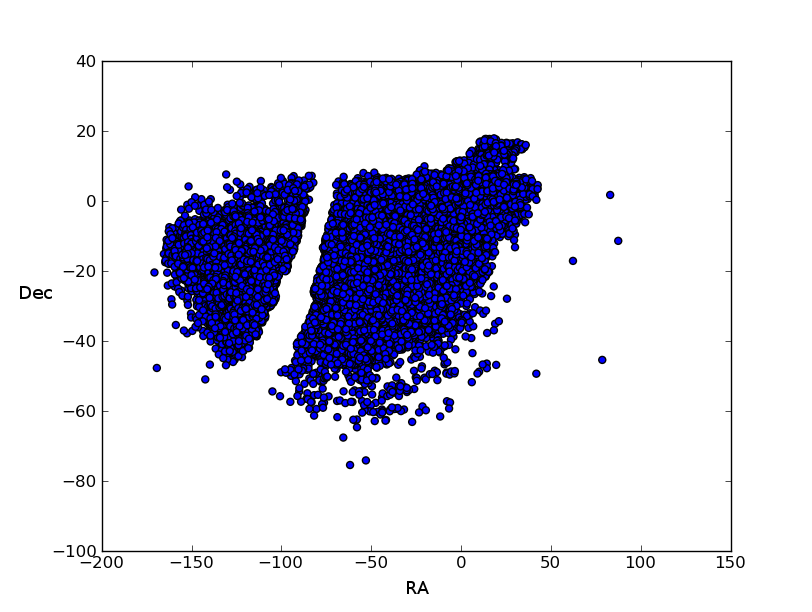
\includegraphics[scale=.7]{newIllustrations/fullSkyYear5_sourcesScatter.png}
\caption[Test diaSource distribution.]{A reduced-density plot of simulated asteroid detections
  (DiaSources) used in our simulated catalog.}
\label{diasPlot}
\end{figure}




\subsubsection{Choosing the Linking Time-Window}

As expected in production, we attempted to generate tracklets between
any pair of images separated by more than 15 minutes and less than
90 minutes.  However, for a more manageable track generation phase, we
attempted to link tracklets if they were separated by $\leq$ 15 days;
in production, it is expected that this number will be 30.  These
numbers should be consistently true across all experiments presented
here.


\subsubsection{Choosing Velocity and Acceleration Limits}
\label{velAccLimits}
\begin{figure}[ht!]
  \centering
  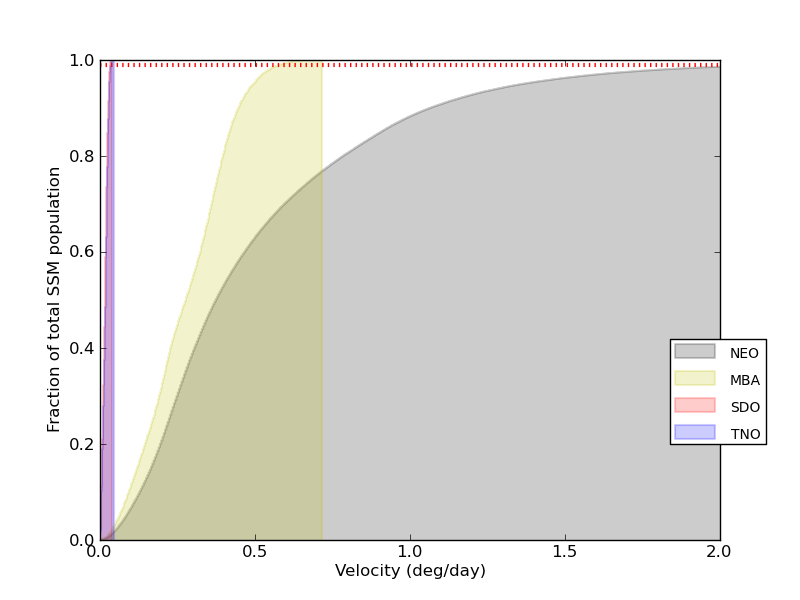
\includegraphics[width=13cm]{illustrations/mopsplots/aug2011/n_velocity.png}
  \caption[Velocity distribution of solar system objects.]{A cumulative histogram of solar solar system object
    sky-plane velocities, organized by classification.  These
    velocities include objects at all solar elongations. Classes of
    objects closer to the Sun and to the Earth (NEOs) move faster than
    objects further away (TNOs). }
  \label{velSurvey}
\end{figure}

\begin{figure}[ht!]
  \centering
  \subfloat[Apparent Accelerations in Right Ascension over 15 Days]{
    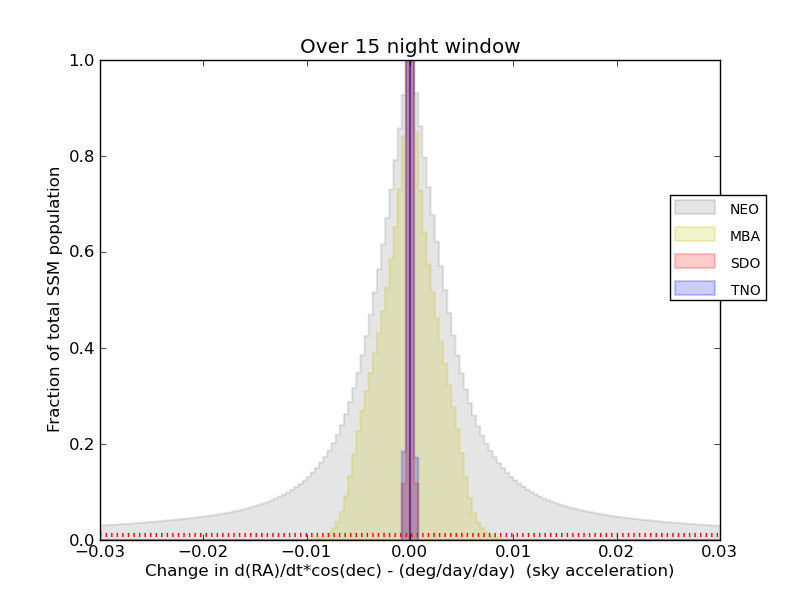
\includegraphics[width=8cm]{illustrations/mopsplots/aug2011/n_accel_ra_15.png}
    }
  \subfloat[Apparent Accelerations in Right Ascension over 30 Days]{
    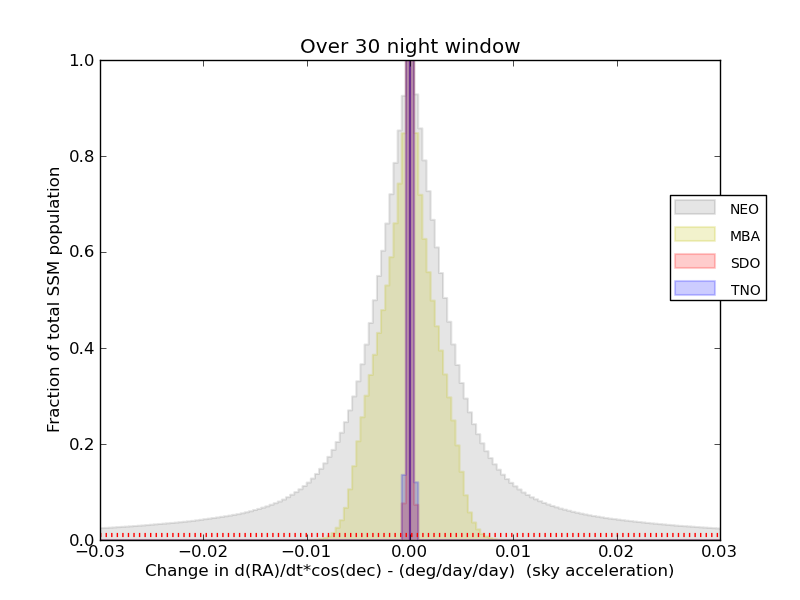
\includegraphics[width=8cm]{illustrations/mopsplots/aug2011/n_accel_ra_30.png}
    }

  \subfloat[Declination Apparent Accelerations in Declination over 15 Days]{
    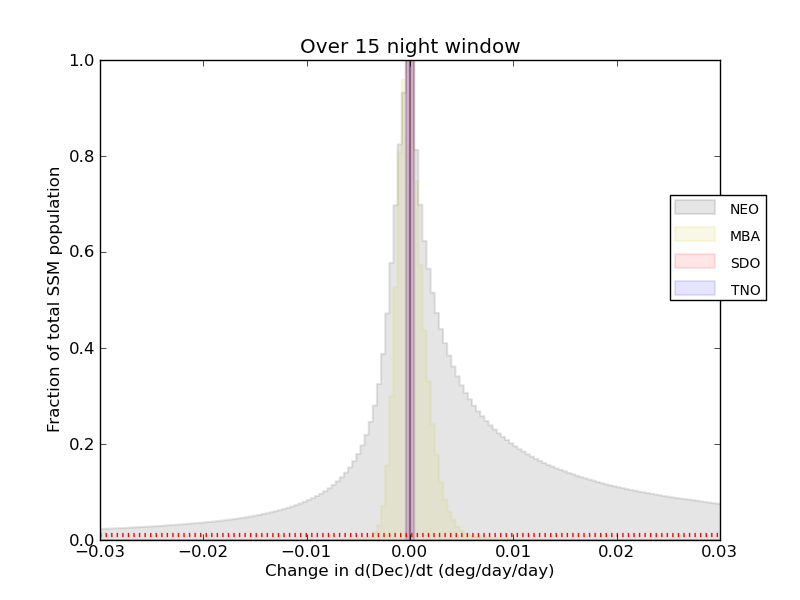
\includegraphics[width=8cm]{illustrations/mopsplots/aug2011/n_accel_dec_15.png}
    }
  \subfloat[Declination Apparent Accelerations in Declination over 30 Days]{
    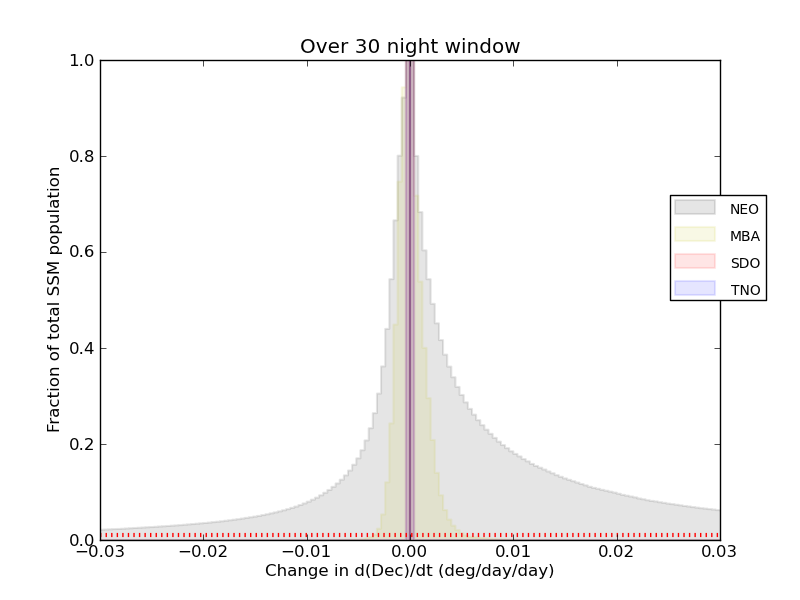
\includegraphics[width=8cm]{illustrations/mopsplots/aug2011/n_accel_dec_30.png}
    }
  \caption[Acceleration distributions of solar system objects.]{Normalized histograms of sky-plane accelerations of several
    classes solar system objects in the RA and declination, with
    objects grouped by classification.  Histograms are presented for
    changes over 15 days and 30 days. The best-fit accelerations vary
    slightly given the size of the window; this is due to
    non-quadratic factors not included in the simple quadratic model.
    15 day tracking windows are used in the experiments presented in
    this document, but we expect to move to 30 day windows in the
    future.  In both cases, virtually all MBAs, and all other objects
    except NEOs, should have accelerations between -.02 and .02
    deg/day$^2$ in both axes.}
  \label{accSurvey}
\end{figure}

We chose limits on velocity and acceleration by looking at the actual
velocities and accelerations of objects from the SSM, after generating
their ephemerides at a variety of times. Histograms of the velocities
and acceleration distributions are shown in Figures~\ref{velSurvey}
and \ref{accSurvey}. 

As can be seen from these distributions, NEOs move fastest and with
the highest accelerations, while outer solar system objects (SDOs,
TNOs) move much more slowly.  In order to detect 99\% of all MBAs,
velocity limits of 0.5 deg/day and an acceleration limit of 
.02 deg/day$^2$ are sufficient. It's worth noting that this is too
slow to detect more than about 60\% of the NEOs, but this is a
simplifying choice made to make find and linkTracklets more manageable
at this stage of development. 

By examining the detections on an object-per-object basis, we
calculated that among the 186,344 objects seen with proper cadence,
186,209 of these (more than 99.9\%) should generate useful tracks
given these velocity and acceleration limits. This is a reflection of
the fact that the overwhelming majority (about 9M of the total 11M)
objects in the SSM are MBAs, while NEOs make up only a small fraction
of solar system objects.

%% see mops64: /mnt/raid/jmyers/variousDensities/fullDensity/maxV.5_15days/trueTracks/*.log

\subsection{Simulation Results}

All simulations were conducted on the Gordon cluster at San Diego
Supercomputing Center.  Because of the large memory requirements for
running MOPS, the vSMP nodes were used for all stages of computation.
Except for the scaling tests, 16 threads were used for all the runs.


\begin{figure}[ht!]
\centering
\begin{tabular}{|r l|}
\hline
Number of asteroid detections: & 36,311,037 \\
Number of non-asteroid detections: & 0 \\
Average detections per night: & 1,134,719 \\
 & \\
Number of tracklets found: & 12,890,181 \\
Number of true tracklets: & 6,859,331 \\
Tracklets \% true: & 53.2\%\\
Tracklet generation time: & 4,791 sec (1.33 hours) \\
Tracklet generation memory use: & 13.7 GB  \\
 & \\
Number of tracks found: & 10,423,382 \\
Number of true tracks: & 5,779,424 \\
Track \% true: & 55.4\% \\
Track generation time: & 36,237 sec (10.1 hours) \\
Track generation memory use: & 16.2 GB \\
 & \\
Number of found objects: & 854,037 \\
Number of findable objects: & 1,128,643 \\
Found / findable: & 75.7\% \\
\hline
\end{tabular}

\caption[Test runs from MOPS run without noise.]{Results from the MOPS run without noise.  Velocity limit was .5 deg/day, acceleration limit was .02 deg/day$^2$ and the track chi squared probability limit was .9.  Note that not quite one fourth of objects which should generate plausible tracks are rejected.}
\label{oneMonth}
\end{figure}

\subsubsection{Survey Efficiency}

Figure~\ref{oneMonth} shows in-depth stats for a `perfect' survey,
where SSM detections above $5\sigma$ SNR in each image are reported
without additional `noise' from artifacts in difference imaging,
background transient or variable objects, or cosmic rays. 
As in all our runs, track generation is far more expensive than
tracklet generation in terms of CPU usage, but both require
substantial amounts of memory.  Also note that nearly one fourth of
the findable objects (those which should generate useful tracks) are
not found. While over time these objects may not be lost forever ({\it
  if} they are discoverable in other apparitions), this is a fairly dramatic
inefficiency in discovery rate, especially when discovery losses due
to survey cadence inefficiencies are considered. The cause of this
inefficiency is not entirely clear at present, however there are
indications it is linked to overly aggressive filtering in the
chi-squared probability filter; examining the pre-determined cutoff,
especially to see if the same cutoff should be applied over the entire
sky, would be a first step. 

Issue: This discovery rate of 75\% is a significant issue for dayMOPS
and should be investigated further. It's possible that simply tuning
the chi-squared probability filter cutoff would fix the problem,
although it could also be related to sky-plane distortion problems
once the poles are included in the input data. 

\subsubsection{Nightly Variance in Runtime}

The cost of running MOPS depends on a variety of factors which are
largely dependent on telescope operations, such as revisit rates and
the locations of revisits.  If no fields are observed that could have
compatible tracklets, then MOPS very quickly rules out these
observations and so runtime is short; on the other hand, if
having lots of potentially compatible detections means that runtime
will be longer. Figure~\ref{nightlyVariance} shows the range of
variations over the month of this simulation. 


\begin{figure}[ht!]
  \centering
  \subfloat{
    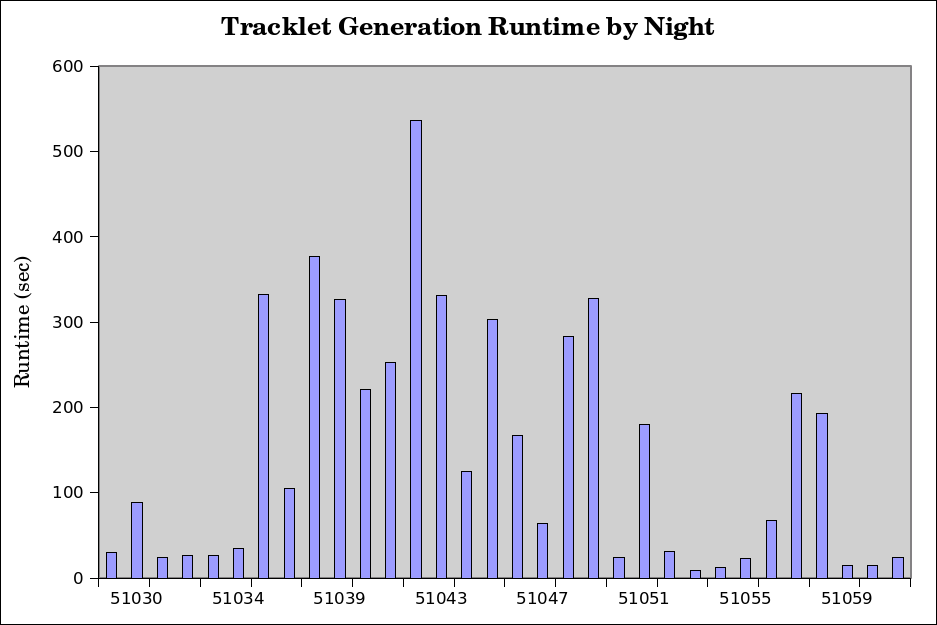
\includegraphics[width=12cm]{newIllustrations/tracklets_nightly.png}
    }
  \\
  \subfloat{
    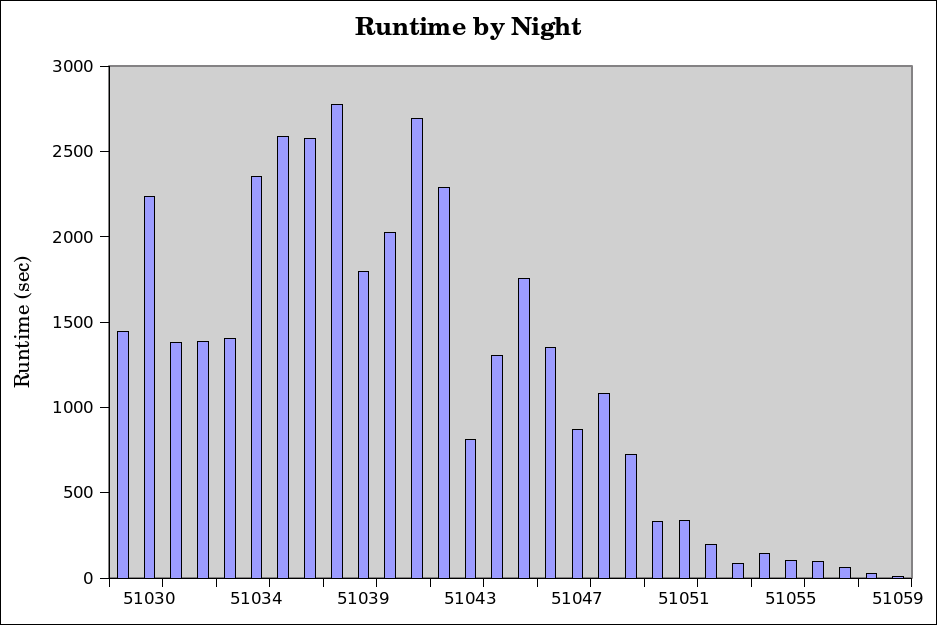
\includegraphics[width=12cm]{newIllustrations/tracks_nightly.png}
    }

  \caption[Compute costs for tracklet and track generation.]{Per-night costs of tracklet generation and track
    generation. Also, in the track generation section,
    note that because only 31 sets of nightly tracklets were
    generated, later runs had less data in their 15-day window and thus ran
    considerably faster.  This is an artifact of the experiment and
    not a meaningful trend.}
  \label{nightlyVariance}
\end{figure}


\subsubsection{Scaling on Non-Asteroid Sources}

Actual images will contain diaSources from non-asteroid sources:
variable stars, supernova, and image processing artifacts (e.g. from
bright stars) will also be present.  Because the quality of image
processing is not known, we added non-asteroid ``noise'' detections to
images at varying rates.  At each rate, a fixed $n$ noise detections
were added to each image, with locations chosen at random. This is not
a truly realistic representation of the noise, as positions of actual
noise sources could be highly correlated and thus mimic actual moving
objects to preliminary stages of linking (thus making compute times
increase). The response of dayMOPS to actual data may thus be quite
different, but this was a reasonable starting point until more
information is available. 

We successfully ran the linking stages of dayMOPS using densities as high as 5,000 non-asteroid
sources per image.  After adding 10,000 non-asteroid sources per
image, tracklet generation was possible but linking tracklets into
tracks was too slow - at over 48 hours for a single night of
searching, it exceeded the wall-clock limit on Gordon jobs.

Figure~\ref{noiseScaling_detections} presents a short summary of the input
detection catalogs generated at each of the noise densities.  For each
of these catalogs, tracklet generation was performed for each of the
31 simulated nights of observation; results can be seen in
Figure~\ref{noiseScaling_tracklets}.  As expected, increasing numbers
of false detections lead to worse-than-linear increases in mislinkage.
This lead to worse-than-linear increases in computational costs for generating the
tracklets, both in terms of CPU and memory usage.

The tracklets generated in the tracklet generation test were used to
test scaling of track generation.  For reasons of time, we only
attempted to search for tracks starting on the first night of
observation ({\it i.e.} the first window of linkTracklets).  Results are presented in
Figure~\ref{noiseScaling_tracks} and Figure~\ref{noiseScaling_found}.
The CPU time cost for track generation scaled worse-than-linearly on
the number of tracklets.  However, we saw only modest increases in the
number of output tracks and runtime for linkTracklets, meaning that we
were able to successfully reject most of these false tracks during
track validation.  Also note that
the number of objects found remained nearly constant across the
various runs.


\begin{figure}[ht!]
\centering

\begin{tabular}{|c c c c|}
\hline
Per-Image Noise Density & Total number of detections & \% noise detections &  \\ 
0             & 36,311,037             & 0\%                          & \\
1,250         & 72,258,537             & 49.7\%          & \\
2,500         & 108,206,037            & 66.4\%          & \\ 
5,000         & 180,101,037            & 79.8\%          & \\
\hline
\end{tabular}
\caption[Input data for runs with noise.]{An overview of the detection sets used for the scaling tests on noise density.}
\label{noiseScaling_detections}
\end{figure}

\begin{figure}[ht!]
\centering

\subfloat[Number of tracklets generated at various noise density levels]
{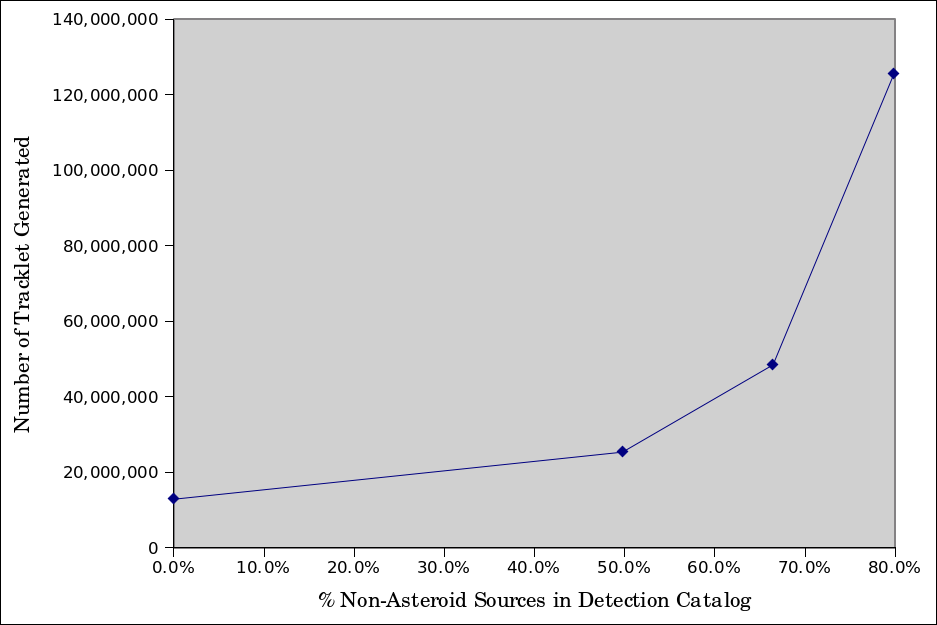
\includegraphics[width=8cm]{newIllustrations/tracklet_num.png}}
\subfloat[Tracklet \% true at various noise density levels]
{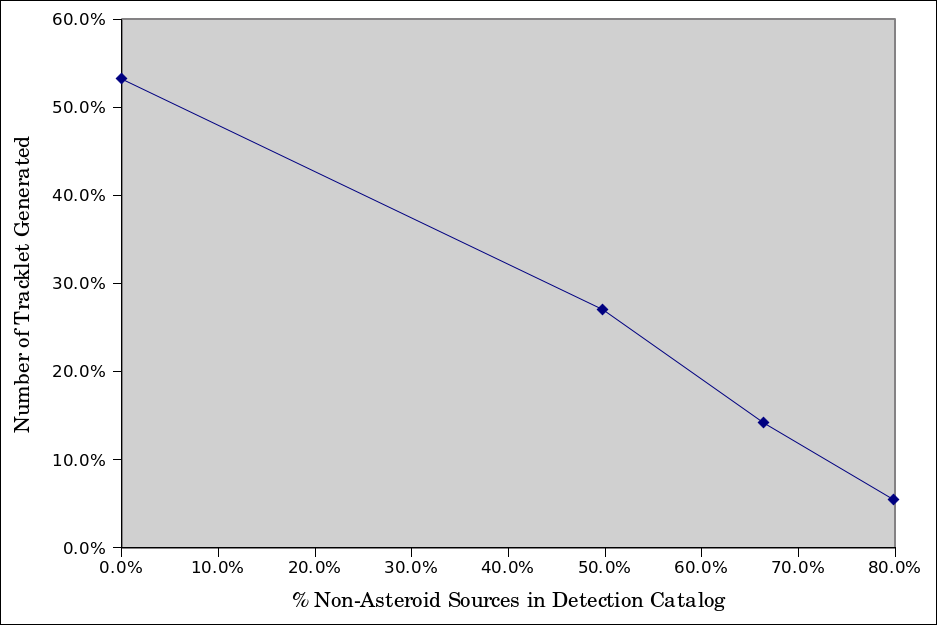
\includegraphics[width=8cm]{newIllustrations/tracklet_true.png}}
\\
\subfloat[Tracklet generation runtimes at various noise density levels]
{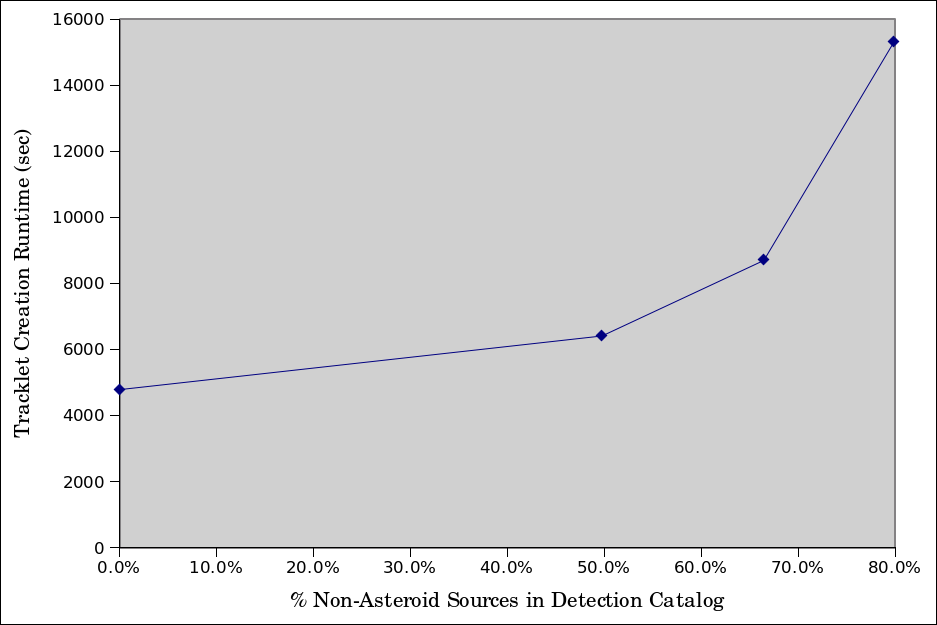
\includegraphics[width=8cm]{newIllustrations/tracklet_runtime.png}}
\subfloat[Tracklet generation memory use at various noise density levels]
{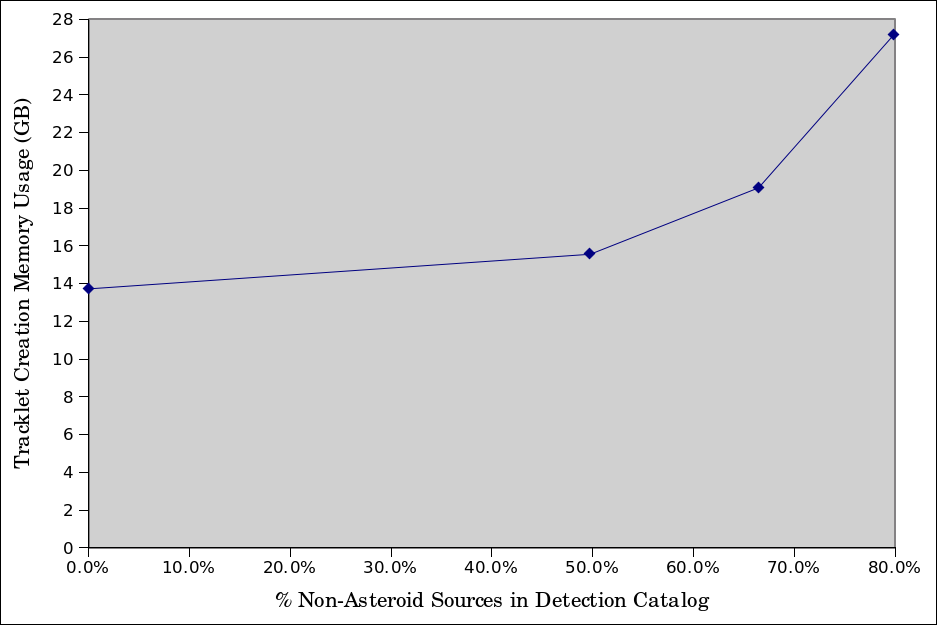
\includegraphics[width=8cm]{newIllustrations/tracklet_mem.png}}

\caption[Tracklet generation for runs with noise.]{Tracklets generated at varying densities of non-asteroid
  ``noise'' sources, and corresponding compute costs.  Each data point
  represents 31 days of tracklet generation.  The same asteroid
  catalog was used for each simulation, but increasing numbers of
  ``noise'' sources were added in each simulation (see
  Figure~\ref{noiseScaling_detections}). Note that the number of
  tracklets generated, and the computational costs to find them,
  increase quickly as noise density increases. This is apparently due
  to the increase of mislinked ``false tracklets''. }
\label{noiseScaling_tracklets}
\end{figure}


\begin{figure}[ht!]
\centering

\subfloat[Number of tracks generated at various noise density levels]
{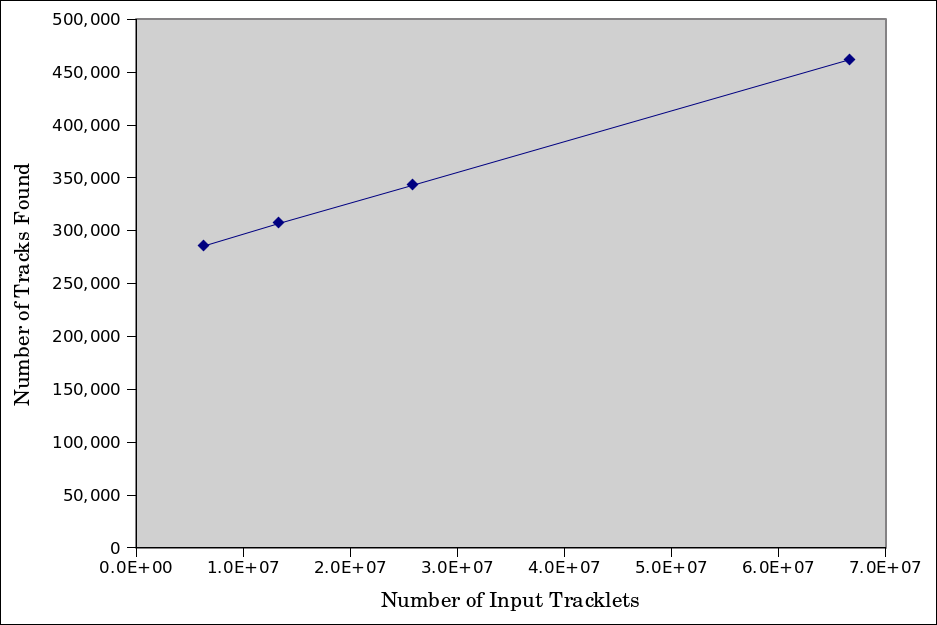
\includegraphics[width=8cm]{newIllustrations/track_num.png}}
\subfloat[Track \% true at various noise density levels]
{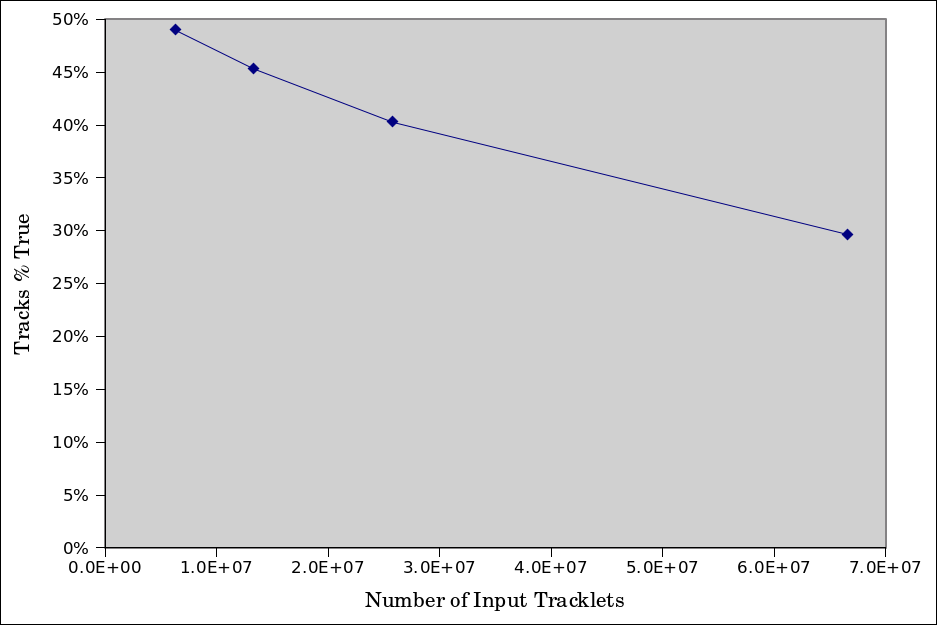
\includegraphics[width=8cm]{newIllustrations/track_true.png}}
\\
\subfloat[Track generation runtimes at various noise density levels]
{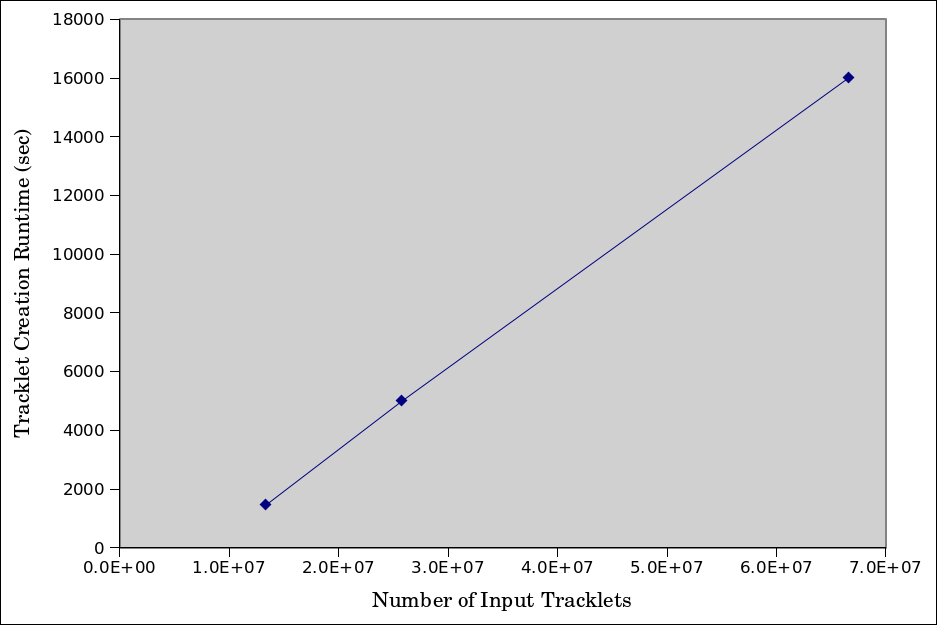
\includegraphics[width=8cm]{newIllustrations/track_runtime.png}}
\subfloat[Track generation memory use at various noise density levels]
{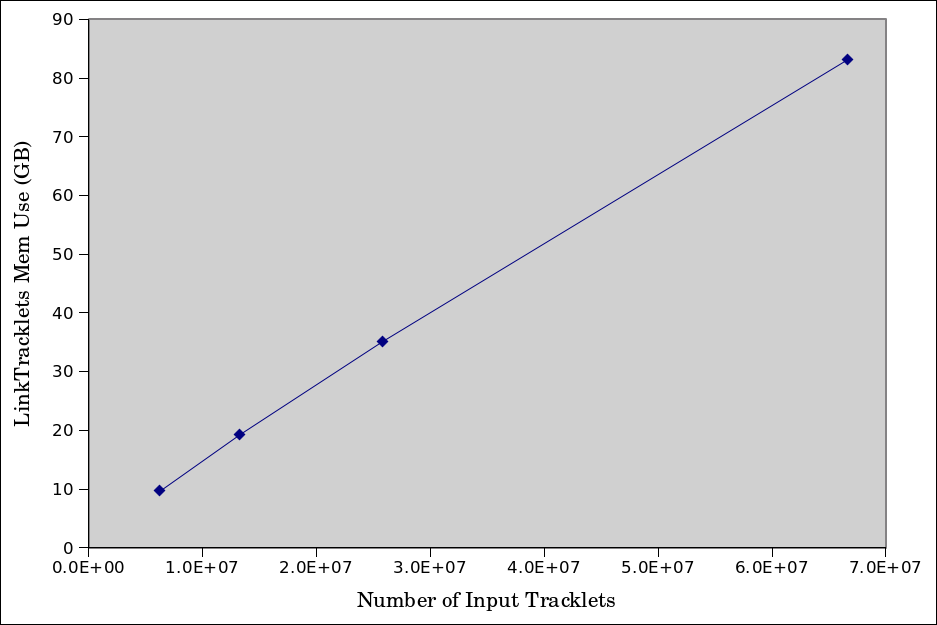
\includegraphics[width=8cm]{newIllustrations/track_mem.png}}

\caption[Track generation for runs with noise.]{Tracks generated at varying densities of non-asteroid
  ``noise'' sources, and corresponding compute costs.  Detections
  catalogs with increasing numbers of noise detections
  (Figure~\ref{noiseScaling_detections}) and tracklets generated from
  these catalogs (Figure~\ref{noiseScaling_tracklets}) were used to generate
  linkTracklets input. For reasons of time, each linkTracklets run
  attempted to find only tracks which started on the first night of
  data and ended anywhere within the first 15 days.}
\label{noiseScaling_tracks}
\end{figure}


\begin{figure}[ht!]
\centering
\begin{tabular}{|c c c|}
\hline

Noise Density & Number of Tracklets & Found Objects \\
0 & 6,312,807 & 55,982 \\
1,250 & 13,318,186 & 55,870  \\
2,500 & 25,824,121 &  55,751  \\
5,000 & 66,635,397 &  55,464  \\
\hline
\end{tabular}

\caption[Test run results for runs with noise.]{Objects found by linkTracklets with varying densities of
  noise in the input catalogs.  Note that the number of objects found
  is only slightly affected by the presence of noise in the input
  catalogs.}
\label{noiseScaling_found}
\end{figure}



\subsection{Conclusions}

For LSST images, we expect that 50-80\% of the DiaSources in our
catalogs may be attributable to non-asteroid, real astronomical sources, before
considering image subtraction artifacts.  This
corresponds to roughly 1250 or 5000 ``noise'' points per image, as we
simulated.

To meet requirements, we must be capable of running one night's-worth
of tracklet generation, track generation (using the entire previous
15 to 30 day window's worth of tracklets), and per-track IOD within 24
hours, plus precovery and attribution.  For the 50\% noise case, we saw a maximum tracklet generation
time of 10 minutes (using 16 CPUs) and for the 80\% noise case we saw
a maximum tracklet generation time of 21 minutes (again using 16
CPUs).  In our testing of track generation, we saw 306,866 tracks and
461,902 tracks generated in the 50\%-noise and 80\%-noise cases
respectively.  Expecting a trivially parallel IOD and an IOD cost of
roughly .001 seconds/track, we anticipate that IOD should not be
problematic: given a few hundred CPUs, we should be able to complete
the nightly IOD processing in a few wall-clock hours.

The cost of running linkTracklets, however, could be problematic given
the 24-hour limit.  As seen in Figure~\ref{noiseScaling_tracks} (c),
linkTracklets can be quite slow, and runtimes can increase
worse-than-linearly on the number of input tracklets, with non-linear
factors becoming significant somewhere between the 50\%-noise and
80\%-noise cases.  In the 50\%-noise experiment, runtime for a single
night was only 1.4 hours, but for the 80\%-noise experiment, runtime
was 32.5 hours!  Again, both experiments used 16 CPUs.  

In our one-month run of linkTracklets without noise, we found the
per-night cost of tracklet generation could vary by a factor of two or
more (see Figure~\ref{nightlyVariance}).  Applying this to the runs performed with noise, this gives us
an estimated maximum nightly runtime of between 2.8 and 65
hours (assuming 16 CPUs).

In order to reach the goal of running tracklet generation, track
generation, and IOD on the tracks, we should aim to reduce the maximum
runtime of linkTracklets to below 20 hours in the worst case.  This
requires a speedup of at least 3-4 over the current performance.  Such
a speedup may be possible simply by waiting on Moore's law, but it would be preferable to begin experimenting with
larger numbers of threads and possible sequential optimizations as
soon as possible, together with looking at potential improvements in
the uderlying KD-Tree algorithms (such as optimizing the tree-walking
code, making sure the leaf-node sizes are appropriate, checking
support node splitting, and ensuring that memory is being accessed
efficiently. It may also be worthwhile to explore GPUs in the context
of parallelization, if trees can be efficiently split between
different machines to reduce individual memory footprint
requirements (such as was attempted with the preliminary work on a
distributed linkTracklets algorithm by Matt Cleveland). 

Preliminary scaling experiments showed little additional speedup when
using more than 16 CPUs, and a possible slowdown as the number of CPUs
exceeded 20.  However, these tests were conducted using a smallish
data set, and should be repeated with a larger one.  Initial tests
were also conducted on Gordon vSMP nodes, which hold only 16 CPUs per
motherboard; this is another possible cause of the poor scaling beyond
16 CPUs, and should be compared with scaling tests on conventional
single-board, large-memory UMA machines.


\section{dayMOPS: Orbits}
\label{orbits}

Orbits are used in a variety of places within dayMOPS (and nightMOPS). We fit orbits (6 parameter Keplerian orbits) to the sets of diasources which make up a track in order to determine which tracks correspond to real moving solar system objects, as the orbit fits provide much tighter constraints on the linkages than the track fits.  After determining an orbit for a movingObject, we identify potential additional detections from both previous observations and future observations by predicting the positions of the movingObject from the orbit, adding those detections to the fit, and re-evaluating the orbit, through the processes of precovery and attribution. We also use orbits and their uncertainties to determine the positions and their uncertainties of known movingObject for nightMOPS. 

Thus, under the general heading of `orbit software' we actually have a variety of needs. These include:
\begin{itemize}
{\item Ephemeris generation. This is software to generate positions, velocities, and magnitudes of moving objects at a particular time from a given orbital element distribution.  This is needed for nightMOPS and for precovery and attribution. }
{\item Orbit propagation. This is software to propagate orbital elements backwards and forwards in time; the resulting changes in the orbital elements can be minor (updating the mean anomaly, for example) but over a longer timespan can be major (changing semi-major axis and eccentricity due to the influence of other planets, for example). This is often bundled with ephemeris generation, but is not necessarily quite the same. This is needed for ephemeris generation, but may also be important for detecting duplicate movingObjects (a single movingObject discovered at two separate times during the survey). }
{\item Initial Orbit Determination. This is software to fit a preliminary orbit to a set of detections, usually only used when there are only a few detections such as when we first discover a movingObject. This is needed for the orbit determination stage of dayMOPS. }
{\item Differential Orbit Determination.  This is software to fit a full orbit to a set of detections, usually incorporating all available observations and leveraging the initial orbit determination fit into a fit that includes error bars. Sometimes IOD and DOD are packaged together in orbit determination software, but mathematically these are usually separate processes with different assumptions on the underlying orbit. For example, IOD may assume that the detections represent an object near perihelion, while DOD may relax that assumption and try to fit for the perihelion location and mean anomaly. }
\end{itemize}

Often all of these capabilities are bound together in a single distributed software package, but this is not necessarily the case. Furthermore, it may be to LSST's advantage to use different packages for different needs, if there are speed differences. For example, ephemeris generation and orbit propagation may be tasks that translate well to GPU architecture, given the repetitious and math intensive nature of the calculations, while IOD and DOD may not due to the individualized nature of each fit. 

\subsection{Orbit packages}

At present, the number of available open-source software packages is limited. OpenOrb, by Mikael Granvik, provides Fortran95 code with limited python interfaces. OrbFit, by Andrea Milani, provides Fortran95 code only. Both of these software packages provide all the functionality above, although with varying disadvantages. There may be other open-source packages available, but these are the main two we have investigated, and seem to be the only two that provide all functionality required for all types of solar system objects. 

One of the main differences between OpenOrb and OrbFit is their approach to IOD, and in particular, DOD. OpenOrb uses statistical ranging while OrbFit is based on geometric orbit fits for DOD.  A extremely simplified description of statistical ranging would be: generate many possible orbits for a particular set of detections and see which one fits the observations the best. This has the advantage that it will (to the limits of the parameter space which is explored) find the best fit orbit, including being able to distinguish between NEOs and MBAs with short observational arcs. It will return a probability distribution function of all likely orbits, even if they are not connected in orbital parameter space. This makes it scientifically most accurate in calculating an orbit, and gives the best estimate of whether an object is truly an NEO or not. It has the disadvantage that it is calculating ephemerides for many possible orbits and comparing those predictions to the observed detections, to see which one 'fits the observations best'. This makes it compute-intensive, and as a result, slow.
An extremely simplified description of geometric orbit fits would be: take the observed detections and fit an ellipse through those detections, using an analytic formula. This has the advantage that it is extremely fast in comparison to statistical ranging and could identify orbits well enough to recover the objects at a later time, even if the orbit determination was incorrect. It has the disadvantage that a single orbit, with (most likely) incorrect errors (because generally the error space is non-gaussian) is returned, and in particular, NEO orbits may be assigned to MBA objects at particular solar elongations.  There is likely also differences in IOD, although these details are less clear (to me). 

OpenOrb's code exceeds 60,000 lines in the main portion of the software, and provides two different python libraries for interacting with this code. One is an f2py library which handles ephemeris generation (with and without errors) and orbit propgation, while another is a custom python interface (which may be out of date, depending on if API changes have occured) for IOD and DOD.  OrbFit's codebase exceeds 160,000 lines, so is also not a simple program (there are multiple ways to find best options for the orbit fit, particularly for short arcs, beyond the simple ellipse). Note that the version of OrbFit being used by PS is not quite the same as the open-source version: Milani rewrote some of the code to be faster. There are no python bindings, and OrbFit interacts with data through text files (separate files for each object). 

A rough comparison of the relative speed of orbit determination using each of these methods gives:
\begin{itemize}
{\item OpenOrb 20s / track (estimates from JM) [10s for ranging (IOD) with a subset of detections, 10s LSL (DOD) with all linked detections] }
{\item OrbFit 0.005s / track (estimates from PS)}
\end{itemize}
Obviously, this difference in orbit fitting is significant. It is likely that the requirements for OpenOrb could be tuned with better understanding of the ranging and least-squares stages, but it seems unlikely that it will be as fast as OrbFit (or even within a few orders of magnitude).  Beyond considerations of the speed of orbit fitting, there are also considerations of ease of use and integration with the LSST stack. This is where OrbFit is difficult, as requiring text files for each object will not scale well for the number of objects expected in LSST or for our computing platform. In addition, it would be difficult for LSST to maintain these codes independently of the original authors. 

Orbit determination is performed per-track and is thus trivially parallelizable. In addition, unlike the linking phases, these algorithms require little memory overhead. 

In terms of ephemeris generation, both packages appear similar. We have done some tests to determine the timing requirements for ephemeris generation with OpenOrb and find 
\begin{equation}
\text{Time}_{10,000\text{\,objects}} (s) \approx 0.7(\frac{s}{\text{day}}) (\text{Days\,from\,Orbit\,Epoch}) + 3.5 (s)
\end{equation}
on a macbook pro (see Figure~\ref{scalingEphemeris}). The major things to note here are that the time required to generate an ephemeris increases as the difference between the orbital epoch and the time of the requested ephemeris increases (due to the need to propagate the orbit to the time of the ephemeris), and that there is some overhead due to reading in the JPL binary files that describe the position of the Earth and other major planets and writing out the outputs. In addition, the time required to generate ephemerides for N objects scales as O(N). 


\begin{figure}[h]
\begin{center}
  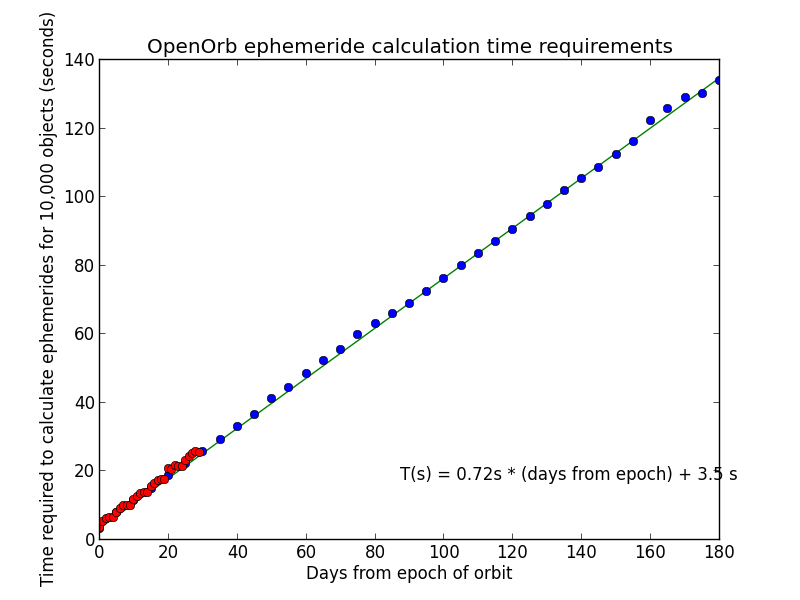
\includegraphics[width=6in]{illustrations/openorb_ephems.png}
\end{center}
\caption[OpenOrb ephemeris computation time requirement.]{Results of a test of the time required to generate ephemerides for 12,078 objects (scaled to 10,000 objects for the plot) using OpenOrb. }
\label{scalingEphemeris}
\end{figure}

\section{Precovery and Attribution}
\label{precoveryattribution}

This section is intended to provide a brief overview of the requirements for precovery and attribution, along with some speculation on how these tasks may be implemented. 

\subsection{Attribution}

Attribution is the process of adding new observations to an existing movingObject, thus increasing its observed orbital arc. This decreases the errors in the orbital parameters, generally making the object more useful for dynamical modeling or studying orbital distributions of populations and making future ephemeris predictions for the object more accurate. These additional observations are particularly useful when the orbital arc is short. 

Attribution could take place by adding single detections within a night, if the ephemeris prediction is suitably low in error and a comparison image or template shows that no other star, galaxy or transient object is present at the predicted location. This process should be considered if the LSST cadence results in many single visits per night, or perhaps as an additional goal to fill in as many observations as possible. However, in general, it will be more reliable to extend the arc by looking for multiple observations of the same moving object within a night, so as to use not only the position but also the velocity as match criteria. This allows larger ephemeris errors to still result in a reliable identification and means that tracklets should be the basis for attribution. 

The process of attribution would then go as follows: 
\begin{itemize}
\item{After the night's worth of observations, dayMOPS findTracklets phase produces tracklets.}
\item{Ephemerides for all the currently known movingObjects are produced, at some intervals over the time span of observing.}
\item{These ephemerides (presumably placed into some form of KD-Tree holding position and velocity information) are compared to the night's tracklets (also placed in a similar KD-Tree), and the intersecting matches are inspected further.}
\item{For each movingObject and tracklet match, take all the detections which make up the movingObject and the tracklet and use these to attempt to fit an updated orbit; if the residuals are appropriate, then the match is considered correct.}
\item{For correct matches, the movingObject orbit is updated, the detections are flagged as belonging to this movingObject, and the detections (and any tracklets involving those detections) are removed from the set of tracklets.}
\item{The remaining set of tracklets are then sent onwards to linkTracklets.}
\end{itemize}

The details of matching the ephemerides and the tracklets have not been worked out. The LSST case is demanding because we expect about 800 observations per night and (towards the end of the survey) 11M known movingObjects; this means it will likely be impractical to brute force things by just predicting the positions of all known movingObjects at all observational times. However, work done in nightMOPS is applicable here as well if the velocities are ignored in the first stages, and only considered when examining potential matches; if the requirement is that potential matches are close to the predicted positions in more than one visit, this essentially includes the velocity condition implicitly. 

\subsection{Precovery}

Precovery is the process of adding old observations (that could not be identified at the time) to an existing movingObject, again increasing its observed orbital arc, although here it is `backward' in time. An additional advantage of precovery is that it reduces the uncertainty in ephemeris predictions without waiting for additional observations, thus presumably making further attribution less time consuming as the ephemeris errors become smaller. Again, the most useful method of precovery will include multiple observations within a night.  

There are many possible approaches to precovery. While attribution should be attempted for all known movingObjects as soon as tracklets are formed, precovery should only be done if a movingObject's orbit is significantly changed by adding new observations (`significantly' meaning that the ephemeris predictions move beyond the region which would have been included in any previous attempts at precovery). Precovery efforts should also be limited to a timespan where the uncertainty in ephemeris predictions permit reliable matches. These two factors suggest that precovery may be best handled on an object-by-object basis, perhaps as follows: 
\begin{itemize}
\item{Using the orbit of the movingObject, generate coarse ephemerides backward in time to the point that the uncertainty in the ephemeride predictions reaches a predetermined threshhold.}
\item{Compare these coarse ephemerides (including the predicted magnitudes) to the location of LSST pointings (and their measured $5\sigma$ limiting magnitudes) to determine visits where the movingObject may be visible.}
\item{For the visits where the movingObject may be visible, retrieve diaSources which do not match other known movingObjects or Objects.}
\item{Compare the diaSources to the ephemeris predictions for each time, looking for multiple potential matches within a night.}
\item{Combine the potential matches and the detections which make up the movingObject, and use these to attempt to fit an updated orbit; if the residuals are appropriate the match is considered correct.}
\item{Update the diaSource table to reflect the new movingObject associations, and update the movingObject orbit with the new parameters.}
\end{itemize}

This is likely to become an iterative process; precovery is performed, additional observations are identified and orbit is updated, making further precovery possible. 

A complication with both precovery and attribution is that with the additional observations, it may become clear that diaSources which were previously associated with the movingObject no longer belong ({\it i.e.} the residuals between the orbit predictions and the location of these diaSources becomes larger than the overall RMS). This will mean that further changes in the association of diaSources will occur, and further evaluation of the orbit may be necessary (which observations should be kept, which should be discarded?).  



\section{Further Development Tasks}
\label{furtherDev}

Though the core algorithms of MOPS have been implemented in
LSST-appropriate style, further research and development are needed.


\subsection{Long Duration Survey Performance}

Current simulations cover fairly short time periods, and therefore
emphasize the problem of initial object discovery.  In the course of
the full survey, we expect that many detected sources will be
attributed to already-discovered objects.  Because initial object
discovery phases are relatively expensive and ephemeris calculation is
relatively fast, we expect that the resource usage of the system will
decline over time, as more objects are discovered and the size of
input catalogs is reduced.  This expectation needs to be verified and
quantified.

Attribution, precovery and Moving Object management and refinement of the
Moving Object table are not yet implemented in LSST-compliant software.
Developing this software should be a significant development task.

To test this software, we will need to generate simulated input
catalogs which span longer time periods.  Improvements in the catalog
generation software at UW (which took place after most of the
simulations presented in this document) should make this possible. 

\subsection{Including Trailing for Near-Earth-Object Searching}

\label{neosTrailing}

Near-Earth Objects tend to have the highest sky-plane velocity.  This
presents a significant challenge; as we increase the maximum velocity
limit of our tracklet generation, the potential for mislinkage
increases significantly, leading to higher numbers of tracklets and
increased costs.  

Fortunately, fast-moving NEOs will generate visible trails in our
images.  By requiring all tracklets to show trails consistent with
their apparent sky-plane velocity, we expect that it will be possible
to filter most false tracklet linkages, thus rendering the problem of
NEO searching manageable.

The ability to filter on trailing is dependent almost entirely on our
ability to correctly identify trails in images.  Currently, the
ability of image processing to detect trails is not well quantified.  To
remedy this, we will need to generate simulated images which include
asteroid trails and send them to image processing; further refinement
of image processing algorithms may be neccesary.


\subsection{Distributed LinkTracklets} 

In case the implicit memory sharing is not sufficient (say, because
distributed shared memory systems do not provide adequate
performance), it may be necessary to write an explicitly distributed
linkTracklets.  This was attempted by a CS Master's student, Matt
Cleveland, working with Prof. Dave Lowenthal.  The design was
well-thought out but complex, leading to slow implementation.  The
distributed version was forked off before a variety of changes to the
serial version were made, and never merged with those changes.

The distributed linkTracklets, the master node held only the tracklets
of the endpoint trees, and the higher levels of the endpoint and
support trees.  The master node would attempt the linking algorithm on
the higher levels of the tree until it reached a terminal point; it
would then attempt to predict the amount of work needed to complete
the linking and save the state of the searching and estimated cost to
a buffer.  Periodically, the work items in the buffer are distributed
to worker nodes, with attention given to load distribution as well as
cache issues, attempting to minimize the amount of data which must be
transferred to worker nodes.


\subsection{Trivial Code Changes}
\paragraph{Reducing Memory Bloat in KD-Tree Libraries}

Because of the size of the data sets in MOPS, memory consumption is a
frequent problem.  Though this cannot necessarily be addressed
exclusively through improvements in software implementation alone, the
overhead could be reduced significantly.

Lack of attention to the memory size in the initial implementation of
the KD-Tree library has resulted in needless memory bloat of the
trees.  Each node uses a series of \texttt{std::vector}s which could
be replaced with pointers or C-style arrays.  On a 64-bit
architecture, \texttt{std::vector} has an overhead of at least 24
bytes, where pointers and fixed-size arrays have an overhead of just 8
bytes.  Currently, KD-Trees use four vectors, meaning an overhead of
96 bytes per node.

Further modification could further reduce the size of KD-Tree nodes;
for instance, rather than storing $k$ in an integer, it could made a
template argument so the constant is ``baked in'' at compile time and
would not need to be stored.  

\paragraph{Removing Critical Sections in Parallel Implementations}
In all the multithreaded software (except linkTracklets), we maintain
a single output vector (or set) to which all threads write.  To
prevent conflicts, these writes must be wrapped in critical sections.
Critical sections impose synchronization costs, which may become
significant when threads execute on separate boards and must
communicate over the network (as in vSMP or other OS-level distributed
shared memory systems).

To reduce overhead, each thread should really maintain its own output
vector, which could be used without any critical section and merged
later, after all worker threads have completed, as is done in linkTracklets.

\subsection{Significant Changes in CollapseTracklets}

\paragraph{Motion Vectors} 
Currently, collapseTracklets parameterizes motion using location,
angle, and velocity.  However, for low-speed objects which have
significant observational error, the angle can be affected by
significant error.  This means that setting a threshold for angle
tolerance can be difficult; if set too low, then tracklets from
slow-moving objects may not be merged, and if set too high, then
tracklets from fast-moving objects may be mislinked.

This problem would likely be less severe if motion angle and velocity
were replaced by per-axis velocity in RA and declination.  However,
after making this change, it will be necessary to develop
experimentally determine some effective thresholds, which can be a
time-consuming process.

\paragraph{Polar Distortion}
When projecting the locations and motion vectors of objects to a
common time, the current collapseTracklets implementation currently
treats celestial coordinates as though they were planar.  This is
fairly effective close to the ecliptic, but near the poles it could be
problematic.  Fixing this should be relatively trivial, but it has not
yet been done.

\paragraph{Exploring Parallelism and Caching of Flags}
As mentioned in \ref{parallelization}, there are several possible
methods for dealing with the per-tracklet ``already merged'' flags.
The current implementation does not explicitly address the issue,
and no attempt has been made to compare various approaches and their
performance.

Currently, there is no explicit caching of the ``already merged''
flags, and all threads modify them without regard for locking.  On a
true large-memory, single-board system, this should be fine:
integer-sized reads should be atomic, meaning no partially-written
results could be read, and only in very unusual cases could a stale
value be read. However, in systems with CC-NUMA systems, likely
including vSMP systems such as SDSC's Gordon cluster, it is possible
that stale reads could occur when threads from the same process
execute on multiple boards.


\subsection{Dealing with Near-Pole Distortion in LinkTracklets}

The math used in linkTracklets to determine acceleration is almost
certain to break down on near-pole cases.  Further, the chi-squared
probability fitting and filtering has not yet been tested heavily off
the ecliptic, much less in cases of near-pole objects, and could
reject true tracks at an increasing rate as it sees objects further
from ecliptic.

To deal with the acceleration pruning near poles, it may be wise to
modify the core piece of code to rotate pairs of nodes to near the
origin at each pruning check; however, this may be too computationally
costly to insert into the ``hot spot'' of the program.  Another
solution would be to abandon celestial coordinates and instead use
full (x,y,z) Cartesian coordinates on a unit sphere.  This will
require new math be used for calculating acceleration and pruning, as
well as for tree construction.  It is unclear how performance will be
affected by the change.

Additional evaluation is needed before it becomes clear whether changes to
the higher-order fitting code and chi squared probability filter will
be needed due to these geometry distrotions.


\subsection{Dense and Clustered Noise}

The rate of false tracklet generation increases worse-than-linearly with
the density of detections. Issues with image processing can lead to
dense clusters of false detections packed in a small area, which can
in turn lead to very large growth in the number of false tracklets. 

Additional experimentation will be needed to determine how severe this
problem could be.  If it becomes an issue, it may be necessary to
identify regions with unusually high rates of (potentially) false detections and
simply remove all detections from this region before the data is fed
to MOPS. It's worth noting that PanSTARRS is implementing a technique
similar to this to deal with high densities of detections. 


\appendix
\section{About the KD-Tree Library}

\section{Helpful Metrics and Software Tools}
\subsection{Studying OpSim}
\subsection{Studying Tracks}




% so jeff larsen gave me a list of references as \bibitems.  our other
% references are bibtex format.  So we now have two bibliographies!
% ugly! hopefully no one will particularly care.
\bibliographystyle{apj}
\bibliography{baseline}

\begin{thebibliography}{99}

%% These came from Jeff Larsen for his intro section
\bibitem[Bode(1802)]{1802QB378} Bode, J.~E.\ 1802, Berlin : In 
der Himburgischen Buchhandlung, 1802.

\bibitem[Chiang and Brown (1999)]{MB} {Chiang}, E.~I. and {Brown}, M.~E. 1999,
      \aj, 118, 1411

\bibitem[Gehrels et al.(1990)]{1990ASPC....8...51G} Gehrels, T., McMillan, 
R.~S., Scotti, J.~V., \& Perry, M.~L.\ 1990, CCDs in astronomy, 8, 51 

\bibitem[Gladman et al. (1998)]{BG} {Gladman}, B. and {Kavelaars}, J.~J.
      and {Nicholson}, P.~D. and {Loredo}, T.~J. and {Burns}, J.~A. 1998, \aj,
      116, 2042

\bibitem[Gural et al.(2005)]{2005AJ....130.1951G} Gural, P.~S., Larsen, 
J.~A., \& Gleason, A.~E.\ 2005, \aj, 130, 1951 

\bibitem[Larson(2007)]{2007IAUS..236..323L} Larson, S.\ 2007, IAU 
Symposium, 236, 323 

\bibitem[Pravdo et al.(1999)]{1999AJ....117.1616P} Pravdo, S.~H., 
Rabinowitz, D.~L., Helin, E.~F., et al.\ 1999, \aj, 117, 1616 

\bibitem[Rabinowitz(1991)]{1991AJ....101.1518R} Rabinowitz, D.~L.\ 1991, 
\aj, 101, 1518 

\bibitem[Shoemaker 
\& Shoemaker(1988)]{1988NASTM4041...52S} Shoemaker, C.~S., \& Shoemaker, E.~M.\ 1988, NASA Tech.~Memo., NASA TM-4041, p.~52 - 54, 4041, 52 

\bibitem[Stokes et al.(2000)]{2000Icar..148...21S} Stokes, G.~H., Evans, 
J.~B., Viggh, H.~E.~M., Shelly, F.~C., \& Pearce, E.~C.\ 2000, \icarus, 148, 21 

\bibitem[Tombaugh(1960)]{1960S&T....19..264T} Tombaugh, C.~W.\ 1960, \skytel, 19, 264 

\bibitem[van Houten et 
al.(1970)]{1970A&AS....2..339V} van Houten, C.~J., van Houten-Groeneveld, I., Herget, P., \& Gehrels, T.\ 1970, \aaps, 2, 339 

\bibitem[Wolf(1892)]{1892AN} Wolf, M.\ 1892, Astronomische 
Nachrichten, 129, 337 

\end{thebibliography}


\end{document}
